% Format teze zasnovan je na paketu memoir
% http://tug.ctan.org/macros/latex/contrib/memoir/memman.pdf ili
% http://texdoc.net/texmf-dist/doc/latex/memoir/memman.pdf
% 
% Prilikom zadavanja klase memoir, navedenim opcijama se podešava 
% veličina slova (12pt) i jednostrano štampanje (oneside).
% Ove parametre možete menjati samo ako pravite nezvanične verzije
% mastera za privatnu upotrebu (na primer, u b5 varijanti ima smisla 
% smanjiti 
\documentclass[12pt,oneside]{memoir} 

\DeclareUnicodeCharacter{0301}{*************************************}
% Paket koji definiše sve specifičnosti master rada Matematičkog fakulteta
\usepackage[latinica]{matfmaster} 

\usepackage{graphicx}

\usepackage{subcaption}

\usepackage{multirow}

\usepackage{textcomp}


\usepackage{amsfonts}
\usepackage{amsmath}

\newcommand{\yolo}{\ensuremath{\,\textrm{YOLO}}}
\newcommand{\bvs}{\ensuremath{\,\textrm{BVS}}}
%
% Podrazumevano pismo je ćirilica.
%   Ako koristite pdflatex, a ne xetex, sav latinički tekst na srpskom jeziku
%   treba biti okružen sa \lat{...} ili \begin{latinica}...\end{latinica}.
%
% Opicija [latinica]:
%   ako želite da pišete latiniciom, dodajte opciju "latinica" tj.
%   prethodni paket uključite pomoću: \usepackage[latinica]{matfmaster}.
%   Ako koristite pdflatex, a ne xetex, sav ćirilički tekst treba biti
%   okružen sa \cir{...} ili \begin{cirilica}...\end{cirilica}.
%
% Opcija [biblatex]:
%   ako želite da koristite reference na više jezika i umesto paketa
%   bibtex da koristite BibLaTeX/Biber, dodajte opciju "biblatex" tj.
%   prethodni paket uključite pomoću: \usepackage[biblatex]{matfmaster}
%
% Opcija [b5paper]:
%   ako želite da napravite verziju teze u manjem (b5) formatu, navedite
%   opciju "b5paper", tj. prethodni paket uključite pomoću: 
%   \usepackage[b5paper]{matfmaster}. Tada ima smisla razmisliti o promeni
%   veličine slova (izmenom opcije 12pt na 11pt u \documentclass{memoir}).
%
% Naravno, opcije je moguće kombinovati.
% Npr. \usepackage[b5paper,biblatex]{matfmaster}

% Pomoćni paket koji generiše nasumičan tekst u kojem se javljaju sva slova
% azbuke (nema potrebe koristiti ovo u pravim disertacijama)
% \usepackage[latinica]{pangrami}

% Datoteka sa literaturom u BibTex tj. BibLaTeX/Biber formatu
\bib{matfmaster}

% Ime kandidata na srpskom jeziku (u odabranom pismu)
\autor{Nikola Grulović}
% Naslov teze na srpskom jeziku (u odabranom pismu)
\naslov{Tehnike augmentacije i kreiranja podataka za detekciju objekata}
% Godina u kojoj je teza predana komisiji
\godina{2022}
% Ime i afilijacija mentora (u odabranom pismu)
\mentor{dr Milena \textsc{Vujošević Janičić}, vandredni profesor\\ Univerzitet u Beogradu, Matematički fakultet}
\komisijaA{dr Mladen \textsc{Nikolić}, vandredni profesor\\ Univerzitet u Beogradu, Matematički fakultet}
\komisijaB{Lester de \textsc{Abreu Faria}, Professor at ITA \& PHD in Microelectronics\\ IPFacens, Sorocaba, São Paulo, Brazil}
% Ime i afilijacija prvog člana komisije (u odabranom pismu)
% \komisijaA{------ \textsc{------}, profesor\\ Univerzitet u Beogradu, Matematički fakultet}
% Ime i afilijacija drugog člana komisije (u odabranom pismu)
% Ime i afilijacija trećeg člana komisije (opciono)
% \komisijaC{}
% Ime i afilijacija četvrtog člana komisije (opciono)
% \komisijaD{}

% Datum odbrane (odkomentarisati narednu liniju i upisati datum odbrane ako je poznat)
\datumodbrane{Septembar, 2022.}

\apstr{
Automatska detekcija i prepoznavanje objekata ima veoma važnu ulogu u svakodnevnom životu.
Jedan od najznačajnijih primera korišćenja detekcije i prepoznavanja objekata je kod autonomne vožnje. 
Da bi se omogućilo efikasno prepoznavanje objekata, koriste se metode mašinskog učenja, na primer neuronske mreže, duboko učenje i metode računarske vizije.
Međutim, da bi se dobili rezultati u skladu sa željenim kvalitetom, obično je neophodna velika količina podataka, velika procesorska snaga i označavanje podataka koje može da bude veoma skupo ili u velikoj meri nedostupno. 
Ovaj rad se bavi metodama za proširivanje podataka, kao i metodama za smanjenje vremena potrebnog za obučavanje modela, u slučaju da velika količina podataka ili velika procesorska snaga nisu na raspolaganju.
U radu se podaci proširuju standardnim augmentacijama i metodama kreiranja novih sintetičkih podataka. 
Korišćenjem transfernog učenja smanjuje se vreme koje je potrebno neuronskim mrežama da nauče glavne karakteristike raspoloživih podataka.
Korišćenjem navedenih metoda dobijaju se poboljšani rezultati u odnosu na trenutno najbolji model za detekciju objekata. Poboljšanja modela se ogledaju u boljoj detekciji i u boljem prepoznavanju objekata.
}

% Ključne reči na srpskom jeziku (u odabranom pismu)
\kljucnereci{veštačka inteligencija, mašinsko učenje, računarska vizija, duboko učenje, digitalna slika, VGG16, YOLO, StyleGAN}

\begin{document}
% ==============================================================================
% Uvodni deo teze
\frontmatter
% ==============================================================================
% Naslovna strana
\naslovna
% Strana sa podacima o mentoru i članovima komisije
\komisija
% Strana sa posvetom (u odabranom pismu)
\posveta{}
% Strana sa podacima o disertaciji na srpskom jeziku
\apstrakt
% Sadržaj teze
\tableofcontents*

% ==============================================================================
% Glavni deo teze
\mainmatter
% ==============================================================================



% ------------------------------------------------------------------------------
\chapter{Uvod}
% ------------------------------------------------------------------------------

% uvod o masinskom
Mašinsko učenje (eng.~\textit{machine learning}) se odnosi na sposobnost mašine da donosi zaključke koristeći dostupne podatke umesto strogo definisanih i kodiranih pravila. Zapravo, mašinsko učenje omogućava računarima da sami uče. 
Rezultati mašinskog učenja posredno se javljaju u svakodnevnom životu, od predviđanja vremenske prognoze do autonomne vožnje.

% problem sa podacima i primer 
Tehnike nadgledanog mašinskog učenja podrazumevaju korišćenje velike količine označenih podataka. 
Međutim, postoji više razloga zbog kojih velika količina označenih podataka nije uvek dostupna. Prikupljanje i obeležavanje podataka je proces koji može biti izuzetno skup ili čak i nemoguć \cite{bengio2007scaling}. Na primer, u oblasti medicine, obeležavanje podataka od strane stručnjaka radiologije je skupo i nije izvodljivo u velikim razmerama \cite{litjens2017survey}. U takvim situacijama, mašinsko učenje ima na raspolaganju samo malu količinu podataka i potrebno je primeniti posebne tehnike i pristupe kako bi se problem dostupnosti male količine podataka, ukoliko je to moguće, prevazišao. 

% resenje : prosirenje skupa podataka
U ovom radu se rešava problem dostupnosti male količine podataka, pri čemu su podaci slike sa obeleženim okvirima objekata. Za rešavanje problema male količine podataka koriste se dva pristupa: proširivanje skupa podataka i transferno učenje (eng.~\textit{transfer learning}).
U radu je opisan postupak proširivanja skupa podataka, pri čemu se podaci proširuju standardnim tehnikama za augmentaciju slika i podacima dobijenim pomoću modela za generisanje sintetičkih slika. 
% prosirivanje podataka nije jedino resenje
Proširivanje skupa podataka navedenim metodama i dalje ne rešava dovoljno dobro problem male količine podataka, u radu su opisane i tehnike transfernog učenja  \cite{zhuang2020comprehensive} na već obučenom modelu za detekciju objekta \cite{bochkovskiy2020yolov4}. 
Korišćenje transfernog učenja ima za cilj da se nauče reprezentacije iz jednog domena i prenesu naučene karakteristike u blisko povezan ciljni domen \cite{brigato2021close, bengio2012deep}.
%takođe metod smanjuje vreme potrebno za učenje modela
Indirektan doprinos korišćenja metoda transfernog učenja je i smanjivanje procesorkse snage potrebne za obuku modela.
% rezultat prosirivanja
Korišćenjem navedenih metoda proširivanja skupa podataka i transfernog učenja, dobija se model sa boljim karakteristikama.


U glavi \ref{section2} je dat kratak pregled modela za detekciju objekata koji se koriste u ovom radu. U glavi \ref{section3} je dat pregled tehnika i generativne suparničke mreže koje se koriste u rešavanju problema male količine podataka, dok u glavi \ref{section4} se opisuju tehnike evaluacije tih modela. U glavi \ref{section5} su predstavljeni eksperimenti i rezultati dobijenih modela. U glavi \ref{section6} su ukratko prikazani problemi sa kojima se ovaj rad susreće, metode njihovog prevazilaženja i moguća dalja unapređenja rešenja.


% ------------------------------------------------------------------------------
\chapter{Detekcija objekata}
\label{section2}
% ------------------------------------------------------------------------------

Računarska vizija (eng.~\textit{computer vision}) je oblast mašinskog učenja, koja se bavi izgradnjom i korišćenjem  sistema za obradu, analizu i interpretaciju digitalnih slika ili video zapisa \cite{ballard1982computer, huang1996computer}.
Detekcija objekata je tehnika računarske vizije, koja za zadatak ima 
da otkrije objekte na slici. Za uspešnu detekciju objekta potrebno je obučiti model na velikoj količini podataka. 
Kako je nekada nemoguće nabaviti dovoljnu količinu podatka, koristi se augmentacija podataka: podaci se proširuju dodavanjem modifikovanih ili sintetički generisanih podataka \cite{shorten2019survey}. 

%Nekada je nemoguće nabaviti dovoljnu količinu podatka koja je potrebna za učenje modela i to predstavlja veliku prepreku u razvoju aplikacija.
% da obihvati drugu sekciju
%Augmentacija podataka je jedna od tehnika koja se koristi za povećanje količine podataka. Podaci se proširuju dodavanjem modifikovanih ili sintetički generisanih podataka \cite{shorten2019survey}. 
%Skup za proširenje deluje kao neka vrsta regularizacije i pomaže u povećanju generalizacije modela \cite{shorten2019survey}.

% #######################################
\section{Razvojni put detekcije objekata}
\label{section2_detekcijaobjekta}
% #######################################

% primer koriscenja, kratak pregled i razvoj dubokog ucenja
Detekcija objekata se koristi u velikom broju aplikacija, kao što su, na primer, autonomna vožnja, robotski vid, video nadzor, itd \cite{zou2019object}. U poslednje dve decenije, napredak u detekciji objekata je prošao kroz dva perioda \cite{zou2019object}: "tradicionalni period detekcije objekata" (pre 2014.~godine), i "period detekcije objekata zasnovan na dubokom učenju (eng.~\textit{deep learning})" (posle 2014.~godine).

% napredak zbog cnn-a
Učinak detekcije objekata je značajno poboljšan zahvaljujući dubokoj konvolutivnoj neuronskoj mreži (eng.~\textit{convolutional neural networks, CNN}), što je dovelo do izuzetnih otkrića.
Razvoj duboke konvolutivne neuronske mreže takođe je omogućio otkrivanje graničnih okvira\footnote{Granični okviri predstavljaju koordinate na delu ili celoj slici u okviru kojih se nalazi prepoznati objekat.} i značajnih delova objekta na slikama \cite{girshick2014rich, ren2015faster, kang2017t, amit2020object}.

% era dubokog ucenja, drugi period, 2 vrsete modela
U eri dubokog učenja, detekcija objekata se može grupisati u dva tipa: \textit{dvostepena detekcija} i \textit{jednostepena detekcija}  \cite{zou2019object}.
% U okviru dvostepene detekcije, prva faza modela se koristi za izdvajanje graničnih okvira, dok se druga koristi za klasifikaciju i dalje preciziranje objekata. Ovakav metod detekcije objekata je relativno spor, ali daje veoma precizne rezultate.
U okviru dvostepene detekcije, prva faza modela se koristi za izdvajanje regiona\footnote{Regioni predstavljaju delove slike koji mogu da sadrže objekte ili delove objekata}, dok se druga koristi za klasifikaciju i dalje preciziranje objekata. Ovakav metod detekcije objekata je relativno spor, ali daje veoma precizne rezultate.
% Modeli jednostepene detekcije objekata odnose se na klasu modela koji preskaču fazu predloga graničnih okvira. Ovakvi modeli zahtevaju samo jedan prolaz kroz neuronsku mrežu i predviđaju sve granične okvire u jednom prolazu na kraju. Ovaj tip modela obično ima bržu detekciju, ali manje je precizan pri otkrivanju i prepoznavanju objekata.
Modeli jednostepene detekcije objekata odnose se na klasu modela koji preskaču fazu predloga regiona. Ovakvi modeli zahtevaju samo jedan prolaz kroz neuronsku mrežu i predviđaju sve granične okvire u jednom prolazu na kraju. Ovaj tip modela obično ima bržu detekciju, ali manje je precizan pri otkrivanju i prepoznavanju objekata.


% #######################################
\section{Model za detekciju objekata VGG16}
% #######################################
% VGG16
Model VGG16 koristi CNN i smatrao se jednim od najboljih modela računarske vizije 2014. godine nakon pobede na takmičenju ILSVR (Imagenet) \cite{simonyan2014very}. Autori ovog modela su posmatrali druge modele i zapazili da povećanjem dubine i koristeći arhitekturu sa manjim konvolutivnim filterima, može doći do poboljšanja performansi. Promena arhitekture se pokazala kao značajno poboljšanje u odnosu na prethodne modele \cite{simonyan2014very}. 

Model VGG16 spada u model jednostepene detekcije i dobio je svoj naziv po šesnaest slojeva koji mogu da uče, dok se celokupna mreža sastoji od trinaest konvolutivnih slojeva, pet slojeva agregacije (eng.~\textit{max pooling}) i tri duboko povezana sloja koji se sumiraju u ukupno dvadeset i jedan sloj. Arhitektura modela VGG16 je data na slici \ref{fig:section2_vgg16}.

% SLIKA OK
\begin{figure}[ht]
    \centering
    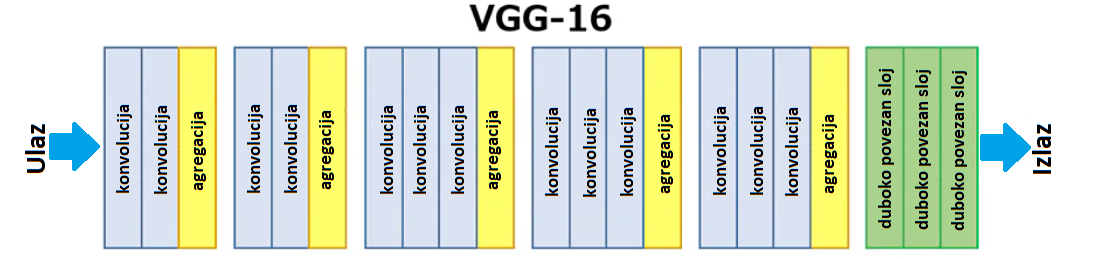
\includegraphics[width=1\textwidth]{matfmaster/glava2/vgg16_2.png}
    % \caption{VGG16 arhitektura \cite{nash2018review}. }
    \caption{VGG16 arhitektura}
    \label{fig:section2_vgg16}
\end{figure}

Model je bio u mogućnosti da predvidi objekte na datim slikama za validaciju sa 6.8\% greške nadmašujući prvi naredni model za 0,9\%. \cite{simonyan2014very}. Nedostatak modela VGG16 je da nije u mogućnosti da odredi okvire detektovanog objekta na slici.



% #######################################
\section{Model za detekciju objekata R-CNN}
% #######################################
% R-CNN , prvi model dvostepene detekcije
% U periodu stagnacije razvoja detekcije objekta (2010.-2012.~godina) dešava se ponovno rođenje konvolutivnih neuronskih mreža \cite{krizhevsky2012imagenet}.
Zbog ponovne upotrebe konvolutivnih neuronskih mreža i veće računarske snage na raspolaganju, 2014. godine pojavljuje se model pod nazivom regioni sa CNN karakteristikama (eng.~\textit{regions with CNN features, (R-CNN)}) \cite{girshick2014rich}. 
Model R-CNN je prvi model dvostepene detekcije i sastoji se od tri modula koji obavljaju različite zadatke \cite{girshick2014rich}:
\begin{enumerate}
  \item Prvi modul generiše predloge regiona pomoću algoritma selektivne pretrage. Algoritam selektivne pretrage vrši segmentaciju slike na osnovu intenziteta piksela koristeći metod segmentacije zasnovan na grafu \cite{narayan2008image}. Na osnovu dobijene mape segmentacije stvaraju se predlozi regiona koji se koriste u sledećem modulu \cite{uijlings2013selective}.
  \item Drugi modul je velika konvolutivna neuronska mreža. Svaki predlog se skalira na sliku fiksne veličine i unosi u obučeni CNN model za izdvajanje vektora karakteristika fiksne dužine.
  \item Treći modul je skup linearnih metoda potpornih vektora (eng.~\textit{support vector machines, (SVM)}) specifičnih za svaku klasu, koji vrše prepoznavanje objekata iz vektora karakteristika.
\end{enumerate}


Problemi koji se javljaju kod R-CNN-a su \cite{gandhi_2018}:
\begin{itemize}
    \item Zbog moguće klasifikacije velikog broja predloga regiona po slici, obučavanje modela nije moguće koristiti u realnom vremenu.
    \item Algoritam selektivne pretrage je fiksiran i kao takav se ne prilagođava podacima. To može da ima za posledicu da se u nekim situacijama dobijaju loši predlozi regiona.
\end{itemize}

% Fast i Faster R-CNN
Tokom nekoliko iteracija razvoja R-CNN-a dolazi do znatnog ubrzavanje modela i time nastaju novi modeli brz R-CNN (eng.~\textit{fast R-CNN}) \cite{girshick2015fast} i brži R-CNN (eng.~\textit{faster R-CNN}) \cite{ren2015faster}.  Model za detekciju objekata brz R-CNN ima sličan pristup kao R-CNN uz nekoliko jednostavnih poboljšanja modela. Model za detekciju objekata brži R-CNN  je sastavljena od dva modula. Prvi modul je duboko povezana konvolutivna mreža koja predlaže regione, dok je drugi modul model R-CNN koji koristi predložene regione za prepoznavanje objekata. Ceo sistem je jedinstvena, ujedinjena mreža za detekciju objekata \cite{ren2015faster}.


% #######################################
\section{Model za detekciju objekata YOLO}
% #######################################
%YOLO
Model za detekciju objekata R-CNN koristi regione da otkrije objekte unutar slike. Model ne gleda na kompletnu sliku, već umesto toga, gleda delove slike koji imaju visoku verovatnoću da sadrže objekte. YOLO (eng.~\textit{you only look once}) je model za otkrivanje objekata koji se razlikuje od modela zasnovanih na regionima. Model YOLO spada u model zasnovan na jednostepenoj detekciji i nastao je 2015.~godine \cite{redmon2016you}. Kod modela YOLO jedna konvolutivna mreža predviđa regione i otkriva objekte u graničnim okvirima.

Odvojene komponente detekcije objekata objedinjuju se u jednu neuronsku mrežu. Model koristi pronađene karakteristike iz cele slike da predvidi svaki granični okvir. Takođe, predviđaju se svi granični okviri za sve objekte na slici istovremeno. To znači da model globalno razmišlja o celokupnoj slici i svim objektima na njoj \cite{redmon2016you}.


% ------------------------------------------------------------------------------
\chapter{Tehnike proširivanja skupa podataka}
\label{section3}
% ------------------------------------------------------------------------------

Skup podataka je moguće proširiti kreiranjem novih podataka. U tehnike za kreiranje podataka spadaju augmentacija podataka i generativne suparničke mreže. U nekim slučajevima i nakon proširenja skupa za obuku, količina podataka koja je na raspolaganju može da bude nedovoljna za obuku modela. Takav problem se može ublažiti tehnikom transfernog učenja. 

% #######################################
\section{Problem malog skupa podataka}
% #######################################
%Da bi se napravio savršen model za detekciju objekata, neophodno je izbalansirati pristrasnost i varijansu.

%Pristrasnost je razlika između predviđenih i pravih vrednosti. Modeli sa velikom pristrasnošću previše pojednostavljuju odnos između predviđene i ciljne promenljive i pokazuju veliku grešku i nad podacima za obučavanje, i nad podacima za validaciju.

%Varijansa odražava varijabilnost predviđanja modela. Modeli sa velikom varijansom obraćaju previše pažnje na podatke za obučavanje i ne generalizuju se dobro nad podacima za validaciju. Kao rezultat toga, ovi modeli pokazuju veoma malu grešku nad skupom za obučavanje i veoma veliku grešku nad skupom za validaciju.

%Modeli sa niskom pristrasnošću i visokom varijansom preklapaju se sa podacima, dok modeli sa velikom pristrasnošću i niskom varijansom ne odgovaraju podacima.

Modeli obučeni na malom skupu podataka teže ka tome da pronađu karakteristike koje ne postoje, što rezultira velikom varijansom i velikom greškom na skupu za validaciju. U ovom radu koriste se dve metode kako bi se izbeglo ovakvo ponašanje. Prvi metod je proširivanje skupa podataka. Podaci se proširuju slikama koje su izmenjene pomoću standardnih metoda augmentacije i slikama koje su sintetički generisane pomoću generativnih suparničkih mreža. Drugi metod predstavlja korišćenje transfernog učenja.

% Kod problema male količine podataka, modeli niske složenosti su se pokazali podjednako dobri ili u nekim slučajevima bolji od modela visoke složenosti. Rezultati su dosta zavisili od dimenzija skupa za obučavanje i upotrebe metoda proširivanja podataka \cite{brigato2021close}.


% #######################################
\section{Standardne metode augmentacije}
\label{section3_increasedata_bas}
% #######################################
U standardne metode augmentacija spadaju rotacija (eng.~\textit{rotation}), refleksija (eng.~\textit{flip}), skaliranje (eng.~\textit{scale}), seckanje (eng.~\textit{crop}), zamućenje (eng.~\textit{blur}) i augmentacija boja (eng.~\textit{color augmentation}).
Nasumičnim kombinovanjem navedenih metoda se kreiraju novi podaci koji služe kao proširenje skupa podataka za obučavanje.

\subsection{Refleksija}
Refleksija slike se odnosi na kreiranje nove slike koja odgovara slici u ogledalu, u odnosu na vertikalnu ili horizontalnu osu. Operaciju refleksije nije moguće primeniti u svakom domenu. Na primer, vertikalna refleksija neće imati mnogo smisla u slučaju saobraćajnih vozila. Primeri refleksije su prikazani na slici \ref{fig:section3_flip}. 

% SLIKA OK 
\begin{figure}[ht]
    \centering
    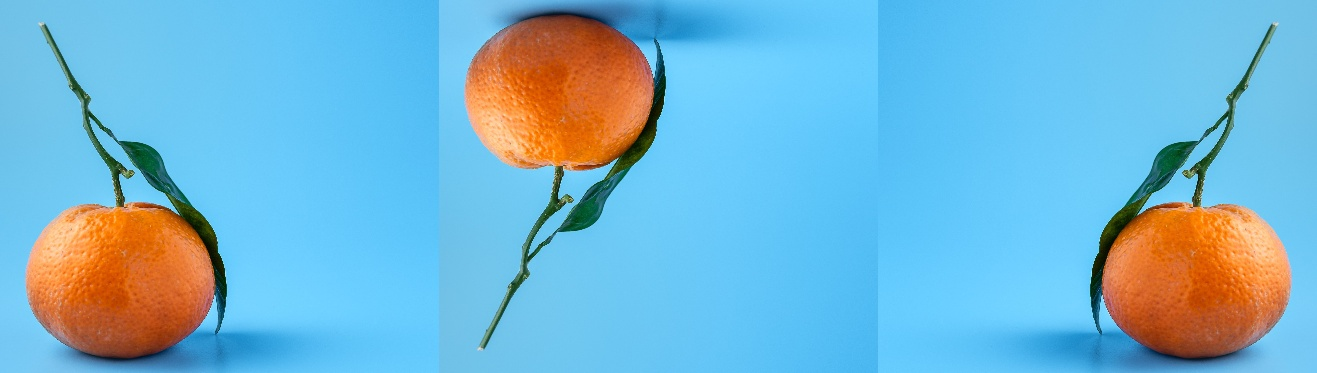
\includegraphics[width=1\textwidth]{matfmaster/glava3/flip.jpg}
    \caption{Primer refleksije: originalna slika (levo), vertikalna refleksija (sredina) i horizontalna refleksija (desno) \cite{unsplashOrange}}
    \label{fig:section3_flip}
\end{figure}

\subsection{Rotacija}
Rotacija predstavlja transformaciju koja kreira nove slike koje odgovaraju originalnoj slici okrenutoj za proizvoljan ugao. Primenom operacije rotacije dimenzije slike se često menjaju. Ukoliko je neophodno sačuvati originalne dimenzije, slika se po potrebi seče, dok se prazni delovi slike popunjavaju određenom metodom. Primeri rotacija su dati na slici \ref{fig:section3_rot}. 


% SLIKA OK 
\begin{figure}[ht]
    \centering
    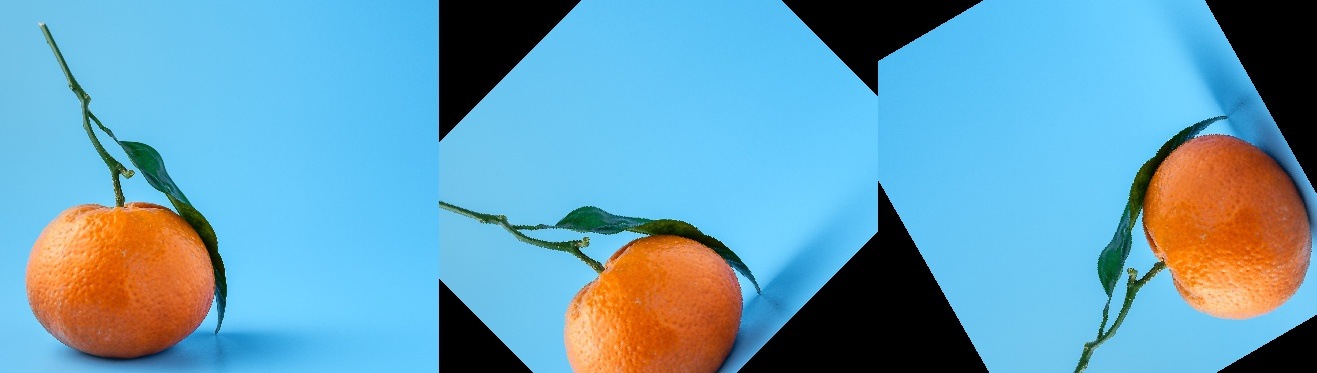
\includegraphics[width=1\textwidth]{matfmaster/glava3/rotate.jpg}
    \caption{Primer rotacije: originalna slika (levo), rotacija za 45\(^\circ\) (sredina) i  rotacija za 120\(^\circ\) (desno) \cite{unsplashOrange}}
    \label{fig:section3_rot}
\end{figure}

\subsection{Skaliranje}
Skaliranje predstavlja transformaciju koja povećava ili smanjuje sliku za zadati faktor koji je veći od nule. Prilikom korišćenja faktora skaliranja većeg od jedan, dimenzije konačne slike su veće od originalne. Da bi se sačuvala originalna dimenzija, nova slika se seče na originalnu dimenziju. U slučaju da je faktor skaliranja između nule i jedinice, dimenzije slike su manje od originalnih. Da bi se sačuvale originalne dimenzije, prazan prostor se popunjava određenom metodom. Primeri skaliranja su dati na slici \ref{fig:section3_scale}.

% SLIKA OK 
\begin{figure}[ht]
    \centering
    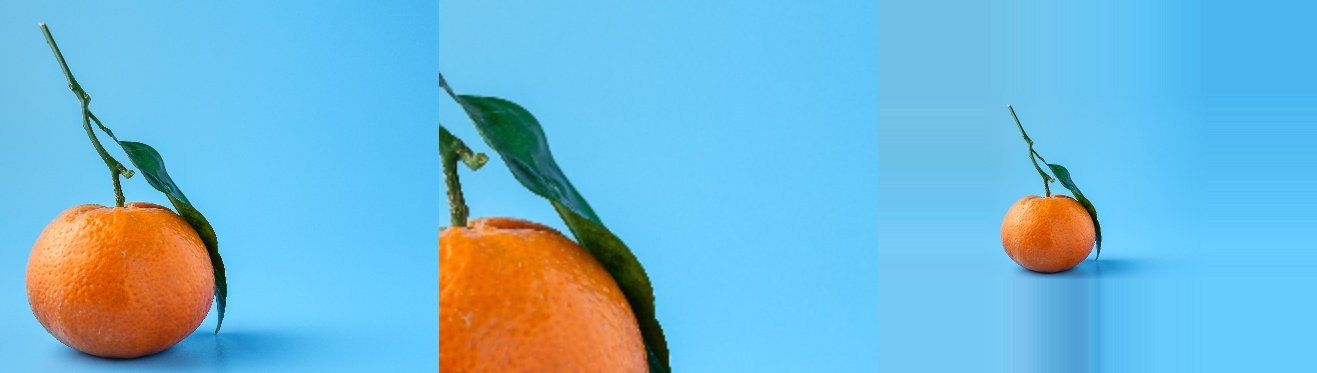
\includegraphics[width=1\textwidth]{matfmaster/glava3/scale.jpg}
    \caption{Primer skaliranja: originalna slika (levo), faktor skaliranja veći od 1 (sredina) i faktor skaliranja između 0 i 1 (desno) \cite{unsplashOrange}}
    \label{fig:section3_scale}
\end{figure}


\subsection{Isecanje}
Isecanje slike se odnosi na kreiranje nove slike nasumičnim uzorkovanjem dela originalne slike. Isečak se potom skalira na dimenzije originalne slike. Primer isecanja je dat na slici \ref{fig:section3_cut}.

% SLIKA OK 
\begin{figure}[ht]
    \centering
    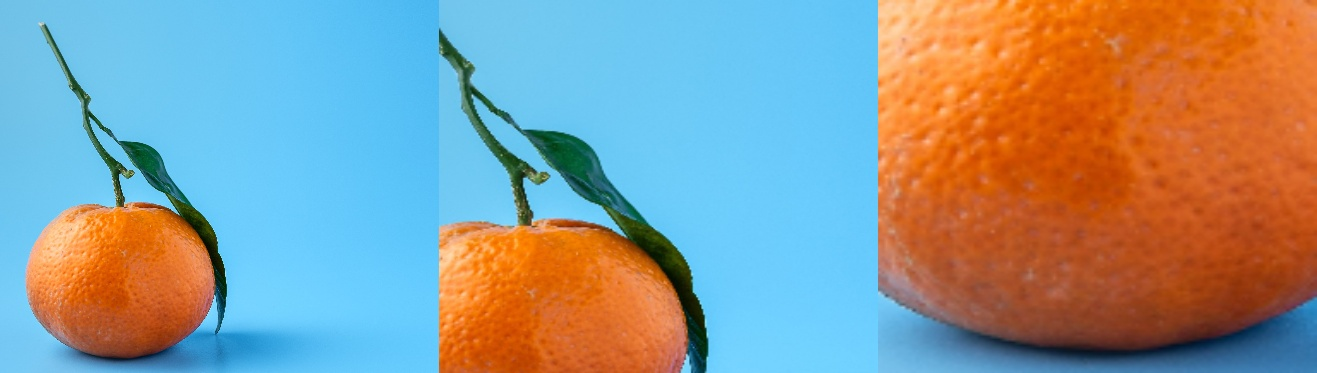
\includegraphics[width=1\textwidth]{matfmaster/glava3/crop.jpg}
    \caption{Primer isecanja: originalna slika (levo), nasumično isecanje (sredina i desno) \cite{unsplashOrange}}
    \label{fig:section3_cut}
\end{figure}

\subsection{Translacija}
Translacija podrazumeva pomeranje slike u horizontalnom ili vertikalnom pravcu. Ovaj metod je veoma koristan, jer se većina objekata može nalaziti na bilo kom mestu na slici. Prazan prostor koji nastaje nakon translacije se boji odgovarajućim metodama. Primer translacije je prikazan na slici \ref{fig:section3_trans}.

% SLIKA OK 
\begin{figure}[ht]
    \centering
    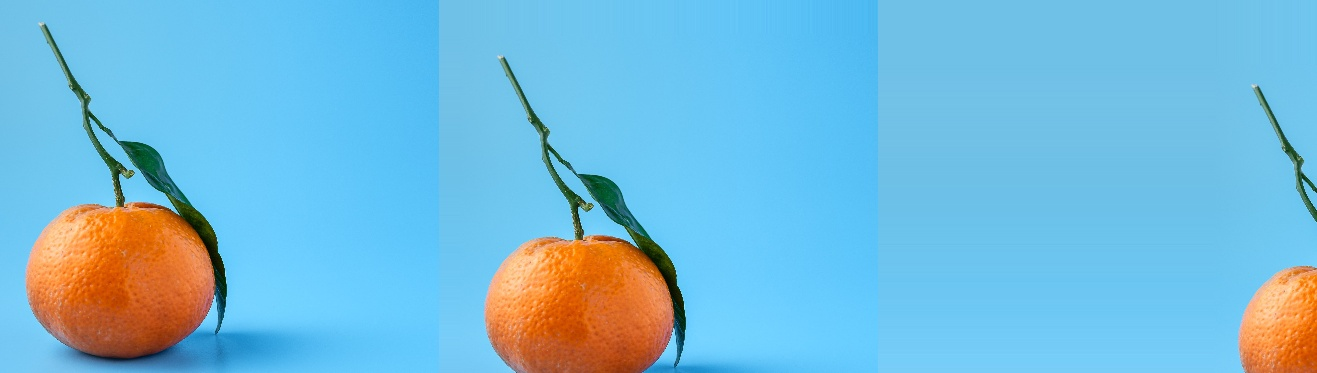
\includegraphics[width=1\textwidth]{matfmaster/glava3/translate.jpg}
    \caption{Primer translacije: originalna slika (levo), nasumična translacija (sredina i desno) \cite{unsplashOrange}}
    \label{fig:section3_trans}
\end{figure}

\subsection{Gausov šum}
Gausov šum predstavlja dodavanje nasumičnih vrednosti iz normalne raspodele na piksele originalne slike. Time se dobija nova slika sa šumom. Dodavanjem Gausovog šuma, deformišu se sve karakteristike u podacima. To je bitno jer u skupu podataka za obučavanje mogu postojati podaci koji sadrže slične karakteristike, što može dovesti do preprilagođavanja modela koji se obučava na tom skupu. Primer šuma je dat na slici \ref{fig:section3_noise}.

% SLIKA OK 
\begin{figure}[ht]
    \centering
    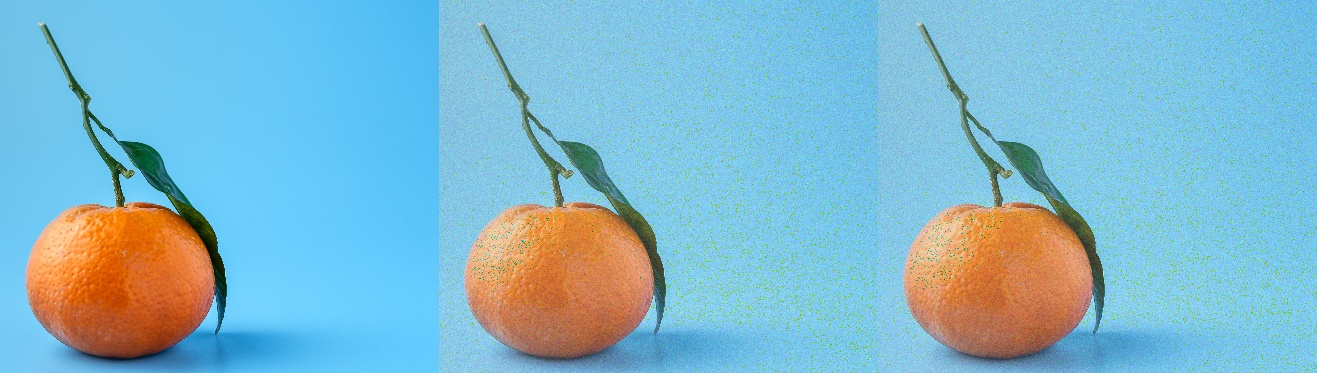
\includegraphics[width=1\textwidth]{matfmaster/glava3/noise.jpg}
    \caption{Primer dodavanja šuma:  originalna slika (levo), srednja vrednost 1 i standardna devijacija 0.1 (sredina), srednja vrednonst 0 i standardna devijacija 0.5 (desno) \cite{unsplashOrange}}
    \label{fig:section3_noise}
\end{figure}

\subsection{Gausovo zamućenje}
Gausovo zamućenje slike predstavlja primenu operacije konvolucije\footnote{konvolucija je operacija nad dve funkcije \(f\) i \(g\) koja proizvodi treću funkciju \(f*g\), koja izražava kako se oblik jedne modifikuje od strane druge} sa Gausovim zvonom \cite{ni2019}.
Povećanjem standardne devijacije dobija se jači efekat zamućenosti. Primer zamućenja je prikazan na slici \ref{fig:section3_blur}.
% \footnote{\( \frac{1}{2\pi\sigma^{2}}e^{-\frac{x^2+y^2}{2\sigma^2}} \)}
% SLIKA OK 
\begin{figure}[ht]
    \centering
    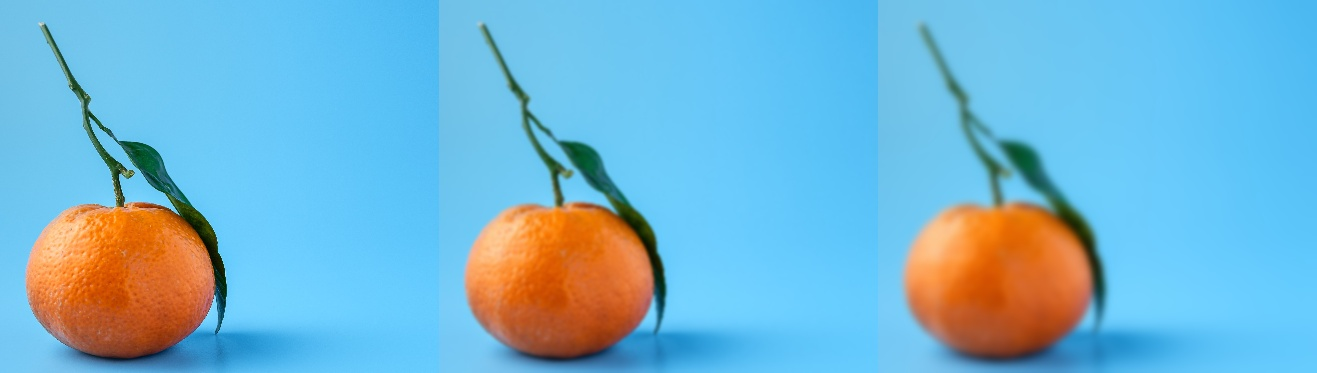
\includegraphics[width=1\textwidth]{matfmaster/glava3/blur.jpg}
    \caption{Primer zamućenja: originalna slika (levo), standardna devijacija 7 (sredina), standardna devijacija 21 (desno) \cite{unsplashOrange}} 
    \label{fig:section3_blur}
\end{figure}


\subsection{Augmentacija boja}

Augmentacija boja (eng.~\textit{color augmentation}) menja svojstava boje slike izmenom vrednosti njenih piksela. Vrednosti piksela mogu se menjati na različite načine.

Tehnika osvetljenja (eng.~\textit{brightness}) podrazumeva množenje svakog piksela slike odgovarajućom faktorom osvetljenja većim od nule. Ako je faktor osvetljenja između nule i jedinice, dobija se tamnija slika, a ako je veći od jedinice dobija se svetlija slika. Primer osvetljenja je prikazan na slici \ref{fig:section3_brightness}.

\begin{figure}[ht]
    \centering
    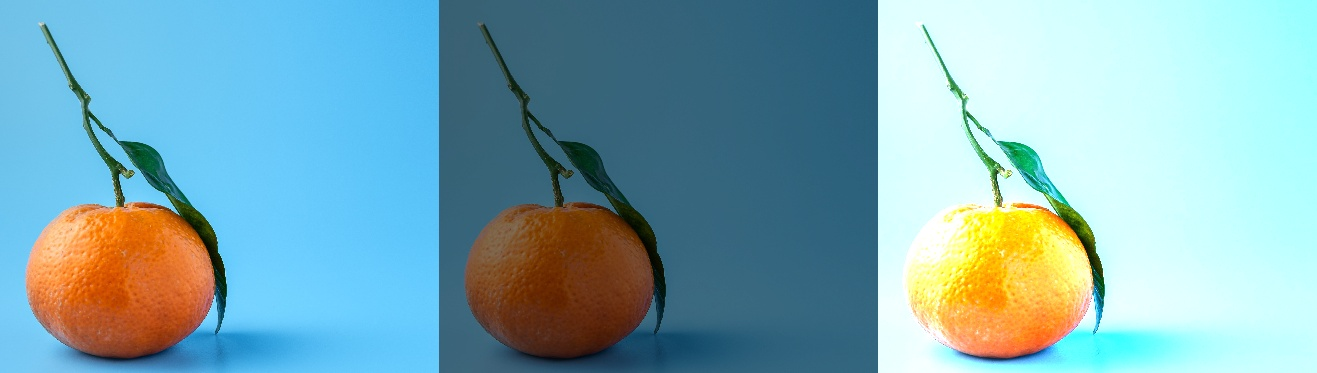
\includegraphics[width=1\textwidth]{matfmaster/glava3/brightness.jpg}
    \caption{Primer menjanja osvetljenja, originalna slika (levo), faktor osvetljenja između 0 i 1 (sredina), faktor osvetljenja veći od 1 (desno) \cite{unsplashOrange}} 
    \label{fig:section3_brightness}
\end{figure}


Tehnika menjanja kontrasta (eng.~\textit{contrast}) predstavlja menjanje stepena razlike između svetlijih i tamnijih delova slike. Povećanjem kontrasta se povećava razlika između svetlijih i tamnijih delova, dok smanjivanjem razlika se umanjuje. Primer promene kontrasta je prikazan na slici \ref{fig:section3_contrast}.

\begin{figure}[ht]
    \centering
    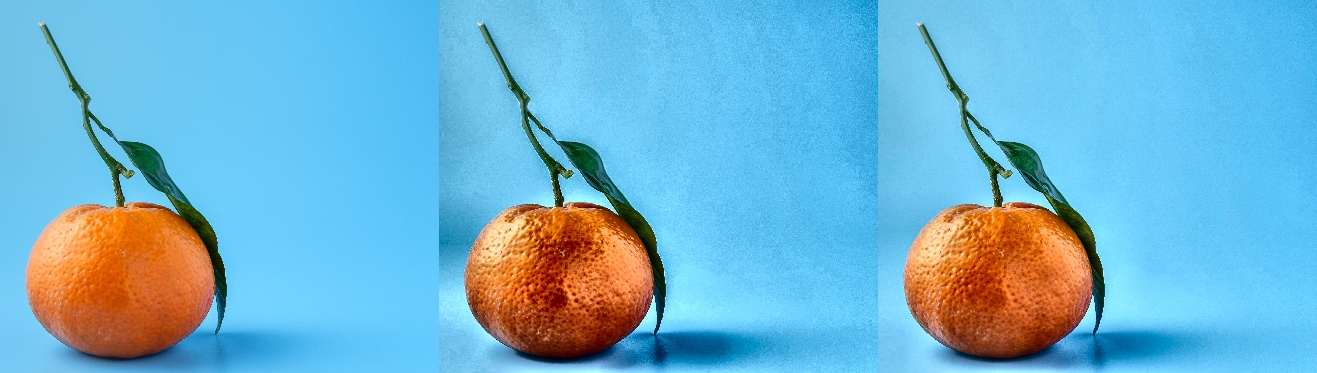
\includegraphics[width=1\textwidth]{matfmaster/glava3/contrast.jpg}
    \caption{Primer promene kontrasta, originalna slika (levo), primer pojačanih kontrasta (sredina i desno) \cite{unsplashOrange}} 
    \label{fig:section3_contrast}
\end{figure}


Tehnika menjanja intenziteta (eng.~\textit{saturation}) slike predstavlja menjanje jačine boja. Povećavanjem intenziteta se dobija slika sa izraženijim bojama. Primer promene intenziteta je prikazan na slici \ref{fig:section3_saturation}.

\begin{figure}[ht]
    \centering
    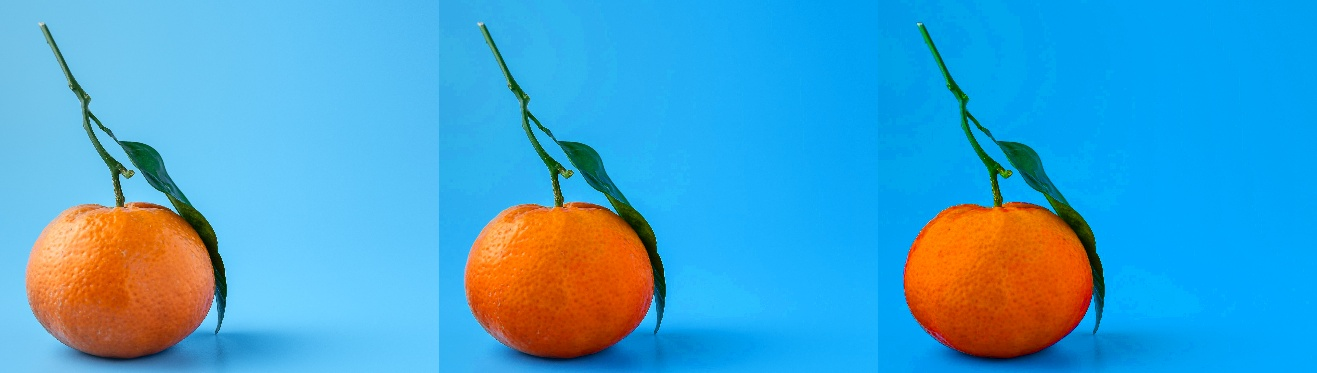
\includegraphics[width=1\textwidth]{matfmaster/glava3/saturation.jpg}
    \caption{Primer promene intenziteta, originalna slika (levo), slabije povećanje intenziteta (sredina), jače povećanje intenziteta (desno) \cite{unsplashOrange}} 
    \label{fig:section3_saturation}
\end{figure}

Tehnika menjanja nijanse (eng.~\textit{HUE}) pomera piksele na slici u drugu tačku na krugu boja. Nasumično pomeranje generiše nove slike sa drugim bojama. Primer promene nijanse je prikazan na slici \ref{fig:section3_hue}.


\begin{figure}[ht]
    \centering
    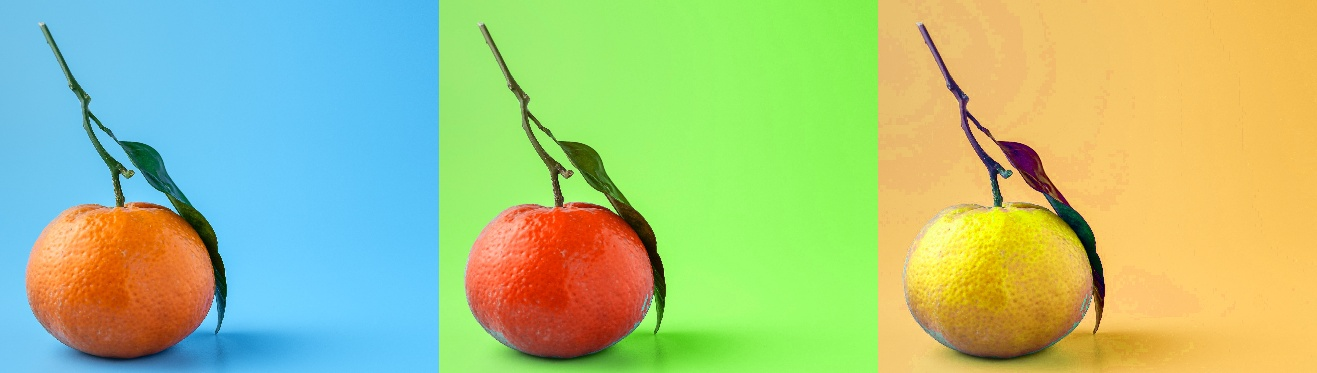
\includegraphics[width=1\textwidth]{matfmaster/glava3/hue.jpg}
    \caption{Primer promene nijanse, originalna slika (levo), pomereni pikseli za nasumične vrednosti (sredina i desno) \cite{unsplashOrange}} 
    \label{fig:section3_hue}
\end{figure}

% #######################################
\section{Generativne suparničke mreže}
\label{section3_increasedata_gan}
% #######################################
%GAN
Tokom razvoja mašinskog učenja, razvijen je koncept generativnih suparničkih mreža (eng.~\textit{generative adversarial network, GAN}). Kod generativnih suparničkih mreža postoje dva modela: \textit{generator} i \textit{diskriminator}. Generator za zadatak ima da generiše slike, a diskriminator da razlikuje slike generisane generatorom od pravih slika \cite{goodfellow2014generative}. Generativne suparničke mreže se u velikoj meri oslanjaju na velike količine raznovrsnih i visokokvalitetnih podataka za obučavanje, kako bi generisali fotorealistične slike \cite{zhao2020differentiable}. Oni nasumično uče i može se reći da je rezultat dobar kada diskriminator ima približnu preciznost od 50\%, tačnije kada počne da nagađa da li je slika prava ili ne. Osnovna arhitektura generativnih suparničkih mreža je prikazana na slici \ref{fig:section2_gans}. 

% SLIKA OK 
\begin{figure}[ht]
    \centering
    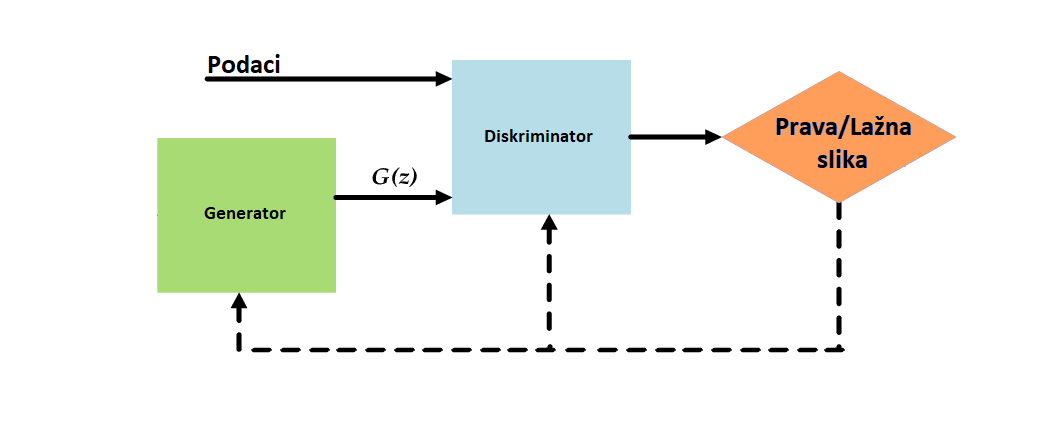
\includegraphics[width=1\textwidth]{matfmaster/glava2/gans_cus.png}
    \caption{Generativne suparničke mreže: ulazni podaci predstavljaju slike, G(z) je generisa slika od strane generatora \cite{gans_image}}
    \label{fig:section2_gans}
\end{figure}

% Progressive GAN
Progresivne generativne suparničke mreže (eng.~\textit{progressive generative adversarial network}) modifikuju arhitekturu na taj način da obučavanje generativnih suparničkih mreža počinje sa niskom rezolucijom slike, a zatim progresivno povećava rezoluciju dodavanjem slojeva u mrežu. Proces obuke je prikazan na slici \ref{fig:section2_augmentation_progressivegans}. Ovakva inkrementalna priroda omogućava da model tokom obuke prvo otkrije vizuelne karakteristike koje se manifestuju na početnim slojevima, od standardnih osobina pa do sitnih detalja \cite{karras2017progressive}.


% SLIKA OK
\begin{figure}[ht]
    \centering
    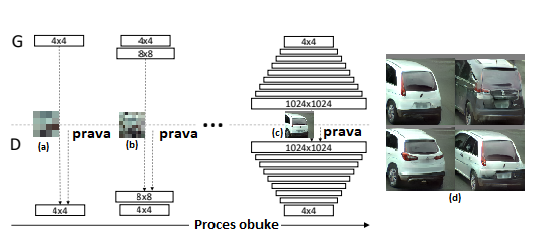
\includegraphics[width=1\textwidth]{matfmaster/glava2/progressive_gan.png}
    \caption{Proces obuke progresivnih generativnih suparničkih mreža počinje od slika niske rezolucije (4\(\times\)4) i progresivno se dodaju slojevi u mrežu i rezolucija povećava do (1024\(\times\)1024). Prva slika (slika a) predstavlja prvu iteraciju obuke modela, druga slika (slika b) predstavlja drugu iteraciju obuke, dok treća slika (slika c) predstavlja poslednju iteraciju. Slike automobila (slika d) predstavljaju generisane slike sa najvećom rezolucijom \cite{karras2017progressive}. }
    \label{fig:section2_augmentation_progressivegans}
\end{figure}

% StyleGAN
Tokom razvijanja generativnih suparničkih mreža najviše se radilo na poboljšanju diskriminatora, što je vodilo ka boljim rezultatima. S` druge strane, \textit{StyleGAN} (eng.~\textit{style generative adversarial network}) je dodatak arhitekturi generativnih suparničkih mreža, koji uvodi značajne modifikacije u model generatora \cite{karras2019style}. 

% generator radi sa latentnim kodom -> ulaz u generator je vektor slucajnih vrednosti -> latentni kod ili z-vektor -> Z -space skup tih vektora -> latentni prostor apstraktnije od z-space
Generator modela zasnovan na stilu se sastoji iz dva dela i prikazan je na slici \ref{fig:section2_augmentation_stylegan}. Prvi deo čini duboko povezanu mrežu sa osam slojeva. Mreža je predstavljena kao funkcija \(f: Z\to W\) i naziva se mreža mapiranja (eng.~\textit{mapping network}). Ulaz mreže predstavlja normalizovani latentni kod \(z \in Z\). Latentni kod (eng.~\textit{latent code}) ili z-vektor \(z\), je vektor koji sadrži slučajne vrednosti iz Gausove raspodele. Prostor u kome se nalaze svi z-vektori se naziva Z-prostor (eng.~\textit{Z-space}) i obeležava se sa \(Z\). Kao izlaz mreže se dobija vektor \(w\) koji pripada latentnom prostoru \(W\). Latentni prostor (eng.~\textit{latent space}) je apstraktni višedimenzionalni prostor koji sadrži vrednosti karakteristika koje se ne mogu direktno interpretirati. Drugi deo generatora predstavlja mrežu koja uz pomoć konstantnog vektora, slučajnog šuma i vektora \(w\) transformisanog afinim transformacijama generiše sliku.

Vektor \(w\) transformisan afinim transformacijama služi za prilagođavanje stila sintetički generisanim slikama pomoću adaptivne normalizacije instance (eng.~\textit{adaptive instance normalization, AdaIN}). Stil slike predstavlja vektor u latentnom prostoru koji je razdvojen od vektora semantičkog sadržaja slike \cite{huang2017arbitrary}. Primer prenosa stila sa jedne slike na drugu je dat na slici \ref{fig:section2_augmentation_adain}.


% SLIKA OK 
\begin{figure}[ht]
    \centering
    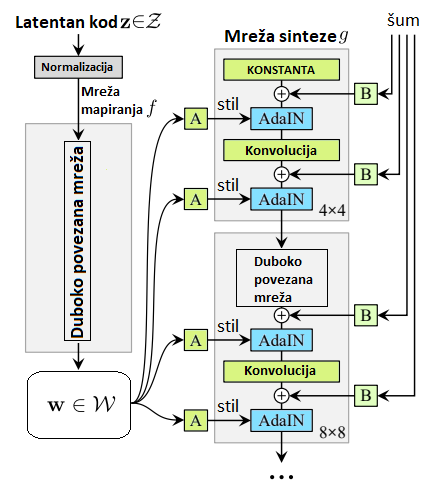
\includegraphics[width=0.8\textwidth]{matfmaster/glava2/stylegan_cus3.png}
    \caption{Model generatora zasnovanog na stilu, "A" predstavlja afine transformacije dok "B" predstavlja faktor skaliranja za šum \cite{karras2019style}. }
    \label{fig:section2_augmentation_stylegan}
\end{figure}

% SLIKA OK 
\begin{figure}[ht]
    \centering
    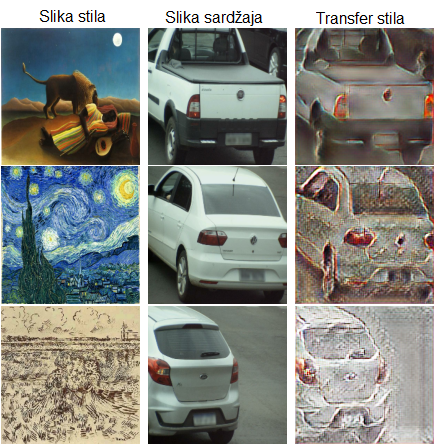
\includegraphics[width=1\textwidth]{matfmaster/glava2/adain_cus.png}
    \caption{Prenos stilova na željene slike i rezultati operacije AdaIN \cite{huang2017arbitrary}. }
    \label{fig:section2_augmentation_adain}
\end{figure}

% StyleGAN2
% \cite{karras2020analyzing}
Model \textit{StyleGAN} generiše fotorealistične slike. Tokom razvoja, model \textit{StyleGAN} je prošao kroz fazu optimizacije i manje izmene mreže sinteze. Nova verzija \textit{StyleGAN}-a, \textit{StyleGAN2} donosi i do 60\% brže obučavanje modela u odnosu na prvu verziju \cite{karras2020analyzing}. Zbog ovakvih ubrzanja, direktno se smanjuje procesorska snaga potrebna za obučavanje. U radu se koristi ova poboljšana verzija, tačnije arhitektura \textit{StyleGAN2}. % Model \textit{StyleGAN2} proizvodi sintetičke slike polazeći od niske rezolucije (4x4), povećavajući je do visoke rezolucije (1024×1024) \cite{karras2020analyzing}.

Ukoliko ne postoji na raspolaganju velika količina podataka, rad sa generativnim suparničkim mrežama može da rezultira nekvalitetnim modelima.
% Problem se javlja kada velika količina podataka nije na raspolaganju i tada obučavanje modela ne dovodi do adekvatnih rezultata. 
Da bi se takav problem ublažio, uvedena je metoda diferencijabilne augmentacije (eng.~\textit{differentiable augmentation}) za model \textit{StyleGAN2}. Metoda koristi različite tipove augmentacija nad stvarnim i lažnim podacima. Metoda omogućava stabilnije obučavanje i dovodi do bolje konvergencije u odnosu na obučavanje modela bez metode diferencijabilne augmentacije nad istim skupom podataka. Model \textit{StyleGAN2} sa metodom diferencijabilne augmentacija je u stanju da proizvede realistične slike, čak i nad skupom podataka koji sadrži samo sto slika \cite{zhao2020differentiable}.
% U stanju je da proizvede realistične slike čak i nad malim skupom podataka \cite{zhao2020differentiable}.


% #######################################
\section{Tehnika transfernog učenja}
\label{section3_trasnferucenje}
% #######################################

U nadgledanom učenju, modeli se obučavaju da nauče odnose koji važe između datih ulaza i izlaza. Modeli zatim mogu da vrše predviđanja izlaza nad novim podacima. Modeli razvijeni na ovaj način davaće bolje rezultate kada rešavaju problem koji se nalazi u istom domenu kao i podaci za obučavanje. Rezultat će se pogoršati ako se domen problema promeni. U najgorem slučaju, može da bude potrebno obučavati novi model čak i kada su domeni problema slični \cite{zhuang2020comprehensive}.

Tehnika transfernog učenja se često koristi kada obuka modela za rešavanje novog problema zahteva veliku količinu resursa. Korišćenje tehnike transfernog učenja donosi niz prednosti od kojih su glavne ušteda resursa i smanjivanje greške tokom obuke modela \cite{zhuang2020comprehensive}. Tehnika transfernog učenja uzima relevantne delove postojećeg naučenog modela i primenjuje ih za rešavanje sličnih problema. 

Tehnika transfernog učenja je jedna od tehnika koja se koristi kako bi se premostio problem nepostojanja dovoljne količine podataka. Transfernim učenjem se prenosi znanje iz postojećeg modela u novi model koji treba da rešava sličan zadatak. Ključni deo transfernog učenja je generalizacija. To znači da se prenosi samo ono znanje koje se može koristiti u drugim  domenima. Umesto da modeli budu čvrsto vezani za skup podataka za obučavanje, modeli koji se koriste u transfernom učenju su opštiji \cite{zhuang2020comprehensive}.




% #######################################
\chapter{Tehnike evaluacije modela}
\label{section4}
% #######################################

Za evaluaciju modela kod detekcije objekta koristi se mera srednje prosečne preciznosti (eng.~\textit{mean average precission, mAP}), koja uzima u obzir preciznost (eng.~\textit{precision}) i odziv (eng.~\textit{recall}). Takođe, koristi se i matrica konfuzije, kod koje računanje ispravno i pogrešno klasifikovanih objekta zavisi od zadatog praga metrike preseka po uniji (eng.~\textit{intersection over union, IoU}) i ocene pouzdanosti (eng.~\textit{confidence score}) klasifikovanih objekata. Ocena pouzdanosti predstavlja vrednost verovatnoće objekta koju joj je model dodelio prilikom klasifikacije.


% +++++++++++++++++++++++++++++++
\section{Presek po uniji}
% +++++++++++++++++++++++++++++++
Za zadatke otkrivanja objekata, preciznost se izračunava pomoću metrike preseka po uniji. IoU je metrika evaluacije koja se koristi za merenje tačnosti detektora objekata na određenom skupu podataka. Na slici \ref{fig:section3_iou} dat je primer okvira, gde je predviđen okvir nacrtan crvenom bojom, dok je pravi okvir nacrtan žutom bojom. Metrika se računa tako što se presek dva okvira podeli sa njihovom unijom (slika \ref{fig:section3_iou_calc}).

% SLIKA OK 
\begin{figure}[!ht]
    \centering
    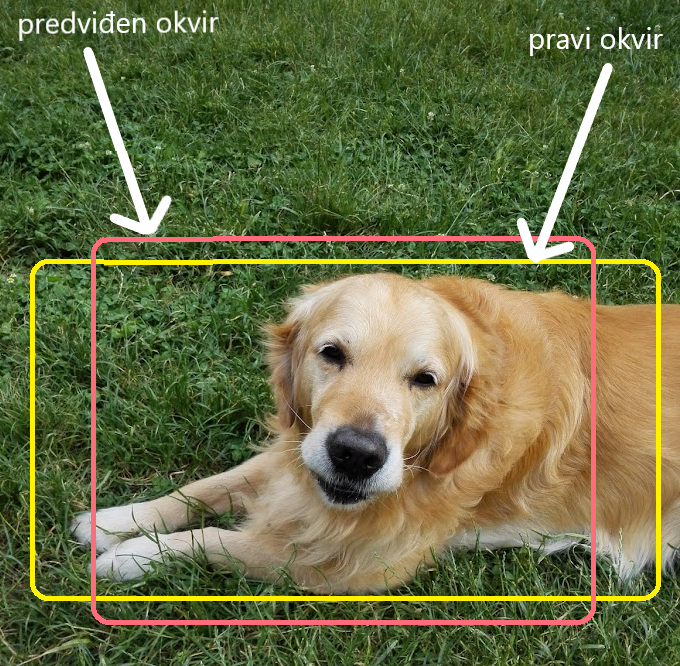
\includegraphics[width=0.7\textwidth]{matfmaster/glava3/iou_cus.png}
    \caption{Predviđen okvir (crveno) i pravi okvir (žuto) nad zadatim objektom}
    \label{fig:section3_iou}
\end{figure}

% SLIKA OK 
\begin{figure}[!ht]
    \centering
    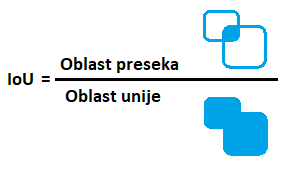
\includegraphics[width=0.5\textwidth]{matfmaster/glava3/iou_calc_cus.png}
    \caption{Demonstracija računanja IoU metrike}
    \label{fig:section3_iou_calc}
\end{figure}



% +++++++++++++++++++++++++++++++
\section{Matrica konfuzije za detekciju objekata}
% +++++++++++++++++++++++++++++++
% bolje objasnjenje
Matrica konfuzije je tabelarni prikaz brojeva ispravno i pogrešno klasifikovanih objekata na osnovu kojih se mogu vršiti ocene modela klasifikacije. Za višeklasnu klasifikaciju detekcije objekata matrica konfuzije se proširuje jednom kolonom i vrstom. Nova kolona služi za zapis broja objekata koji su klasifikovani na slici, a na njoj se ne nalaze. Vrsta služi za zapis broja objekata koji se nalaze na slici, ali nisu klasifikovani. Objekti se klasifikuju ispravno ili pogrešno i na osnovu IoU praga (obično se u praksi koristi 0.5) i praga ocene pouzdanosti.

Matrica kofnuzije se računa i za svaku klasu pojedinačno i slična je binarnoj klasifikaciji. Prilikom računanja matrice konfuzije, posmatra se jedna konkretna klasa i ta klasa se smatra pozitivnom, dok skup koji sadrži sve objekte ostalih klasa se smatra negativnom klasom. Ocena pouzdanosti ne učestvuje u računanju matrice konfuzije za svaku klasu.

% Stvarno pozitivan (eng.~\textit{True Positive, TP}) objekat je pozitivan i model ga je klasifikovao kao pozitivnog. Takođe IoU vrednost objekta je veća od zadatog praga.
\textit{Stvarno pozitivni} (eng.~\textit{True Positive, TP}) je broj objekata koji pripadaju pozitivnoj klasi i model im je dodelio pozitivnu klasu. Takođe, IoU vrednost svakog objekta je veća od zadatog praga.

\textit{Stvarno negativni} (eng.~\textit{True Negative, TN}) je broj objekata koji ne pripadaju pozitivnoj klasi i model im nije dodelio pozitivnu klasu. IoU se ne računa, jer ako objekti ne postoje, neće postojati ni njihovi granični okviri.

\textit{Lažno pozitivni} (eng.~\textit{False Positive, FP}) je broj objekata koji pripadaju negativnoj klasi ali im je model dodelio pozitivnu klasu. Takođe, to mogu biti objekti koji pripadaju pozitivnoj klasi i model im je dodelio pozitivnu klasu, ali IoU vrednost svakog objekta ne prelaze zadati prag.

\textit{Lažno negativni} (eng.~\textit{False Negative, FN}) je broj objekata koji pripadaju pozitivnoj klasi a model im je dodelio negativnu klasu. IoU se ne upoređuje sa pragom jer je klasifikacija pogrešna. 

% +++++++++++++++++++++++++++++++
\section{Preciznost, odziv i \texorpdfstring{$F_1$}{TEXT}-mera}
% +++++++++++++++++++++++++++++++
Preciznost je procenat stvarno pozitivnih objekata među objektima koji su klasifikovani kao pozitivni i definiše se formulom:

\begin{equation}
    Precision = \frac{TP}{TP+FP}
\end{equation}
Veća preciznost takođe znači da postoji manji broj lažno pozitivnih objekata.

Odziv predstavlja procenat pozitivnih objekata koji su ispravno klasifikovani i definiše se formulom:

\begin{equation}
    Recall = \frac{TP}{TP+FN}
\end{equation}

Visok odziv znači da postoji mali broj lažno negativnih objekata.

Preciznost i odziv se mogu sumirati u meru, koja se zove $F_1$-mera (eng.~\textit{$F_1$-score}) i definiše se formulom:
\begin{equation}
\label{eq:f1}
    F_1 = 2\frac{Precision \cdot Recall}{Precision+Recall}
\end{equation}

Srednja $F_1$-mera ili (eng.~\textit{macro-averaged $F_1$-score}) računa se kao aritmetička sredina:
\begin{equation}
\label{eq:f1a}
    F_{1avg} = \frac{1}{n}\sum_{k=0}^{k=n-1} F_{1k}
\end{equation}
gde je \(F_{1k}\) vrednost $F_1$-mere za \(k\)-tu klasu.

Srednja težinska $F_1$-mera se računa sledećom formulom:
\begin{equation}
\label{eq:f1wa}
    F_{1wavg} = \frac{1}{n}\sum_{k=0}^{k=n-1} (F_{1k} S_{k})
\end{equation}
gde su \(F_{1k}\) i \(S_{k}\) vrednost $F_1$-mere i ukupan broj instanci u \(k\)-toj klasi.

% +++++++++++++++++++++++++++++++
\section{Srednja prosečna preciznost}
\label{section4_avgprecision}
% +++++++++++++++++++++++++++++++

Prosečna preciznost (eng.~\textit{average precision}) je način računanja površine ispod krive preciznosti i odziva za jednu klasu. Vrednosti preciznosti i odziva se računaju za zadate vrednosti IoU pragova iz intervala [0.5 do 1.0), najčešće sa korakom 0.05.
Niz izračunatih vrednosti odziva i preciznost se dopunjuje sa \textbf{0} i \textbf{1}, respektivno. 
% Pre računanja, važno je dodati vrednosti \textbf{0} i \textbf{1} na već  izračunatih odziva i preciznosti sa \textbf{0} i \textbf{1}, respektivno. 
Prosečna preciznost se računa sledećom formulom:
\begin{equation}
\label{eq:ap}
    AP = \sum_{k=0}^{k=n-1} (R_{k} - R_{k+1})P_{k}
\end{equation}
gde su \(R_{k}\) i \(P_{k}\) odziv i prezicnost za \(k\)-ti IoU prag.
Srednja prosečna preciznost se računa kao srednja vrednost svih prosečnih preciznosti koja je data formulom:
\begin{equation}
\label{eq:map}
    mAP =\frac{1}{N} \sum_{i=1}^{N} AP_{i}
\end{equation}
gde \(N\) predstavlja broj klasa, a \(AP_{i}\) prosečnu preciznost za klasu 
\(i\).

% +++++++++++++++++++++++++++++++
\section{Fréchet-ova udaljenost}
% +++++++++++++++++++++++++++++++

Fréchet-ova udaljenost (eng.~\textit{Fréchet inception distance, FID}) je metrika koja se koristi za procenu kvaliteta slika koje su generisane od strane generativnih suparničkih mreža \cite{heusel2017gans}. Fréchet-ova udaljenost upoređuje distribuciju generisanih slika sa distribucijom stvarnih slika koje su korišćene za obuku generatora. Fréchet-ova udaljenost za dve iste slike daje vrednost nula, dok za različite daje broj koji je veći od nule.  

Fréchet-ova udaljenost se računa za dve zajedničke normalne raspodele \(\mathcal{N}(\mu,\Sigma)\) i \(\mathcal{N}(\mu',\Sigma')\) sledećom formulom \cite{dowson1982frechet}:
\begin{equation}
    d_{F}(\mathcal N(\mu, \Sigma), \mathcal N(\mu', \Sigma'))^2 =
        \| \mu - \mu' \|^{2}_{2} + 
        tr\left(\Sigma + \Sigma' -
        2\left(\Sigma^\frac{1}{2} \cdot \Sigma' \cdot \Sigma^\frac{1}{2} \right)^\frac{1}{2} \right)
\end{equation}

U praktičnoj upotrebi, distribucije slika se dobijaju računanjem srednjih vrednosti (\(\mu\), \(\mu'\)) i matrica kovarijansi (\(\Sigma\),\(\Sigma'\)) pomoću vektora dobijenih modelom \textit{InceptionV3}\footnote{InceptionV3 je konvolutivna neuronska mreža koja se koristi za analizu slika i detekciju objekata.}. %Funkcija \(tr\) predstavlja trag matrice\footnote{Trag matrice predstavlja zbir elemenata na glavnoj dijagonali kvadratne matrice i obeležava se sa \(tr\)}.


% +++++++++++++++++++++++++++++++
\section{Funkcija greške za generativne suparničke mreže}
% +++++++++++++++++++++++++++++++
Funkcije grešaka za generativne suparničke mreže mogu se formulisati preko igre nulte sume \cite{goodfellow2020generative, hodgson2006microeconomics}. Generator pokušava da minimizuje funkciju dok diskriminator pokušava da maksimizuje. Za dati generator $G$ i diskriminator $D$ problem igre nulte sume se definiše kao \cite{goodfellow2020generative, ml2019}:

\begin{equation}
   \min_{G}\max_{D}\mathbb{E}_{x}[\log{D(x)}] +  \mathbb{E}_{z}[1 - \log{D(G(z))}]
\end{equation}
U datoj formuli:
\begin{itemize}
    \item $D(x)$ predstavlja procenu diskriminatora da je pravi podatak $x$ stvaran,
    \item $\mathbb{E}_{x}$ je očekivanje po raspodeli stvarnih podataka,
    \item $G(z)$ je izlaz generatora za vrednost $z$ iz latentnog prostora,
    \item $D(G(z))$ predstavlja procenu diskriminatora da je lažni podatak stvaran,
    \item $\mathbb{E}_{z}$ je očekivanje po raspodeli podataka u latentnom prostoru.
\end{itemize}

\noindent Funkcija greške za generator se definiše sa:
\begin{equation}
\label{eq:generator}
    \min\log{(1-D(G(z)))}
\end{equation}
i za diskriminator sa:
\begin{equation}
\label{eq:discriminator}
    \max\log{D(x)}+\log{(1-D(G(z)))}
\end{equation}

% Funkcija greške diskriminatora nastoji da maksimizuje vrednost verovatnoće da diskriminator tačno klasifikuje pravu sliku i vrednost logaritma inverzne verovatnoće za lažne slike \cite{goodfellow2020generative}. Funkcija greške za diskriminator se definiše kao:
% \begin{equation}
% \label{eq:discriminator}
%     \max\log{D(x)}+\log{(1-D(G(z)))}
% \end{equation}
% Ova funkcija greške se još naziva logistička funkcija greške.

% Generator minimizuje logaritam inverzne verovatnoće koju predviđa diskriminator za lažne slike. Ovakva funkcija podstiče generator da generiše slike za koje je mala verovatnoća da su lažne \cite{goodfellow2020generative}. Funkcija greške za generator se definiše kao:
% \begin{equation}
% \label{eq:generator}
%     \min\log{(1-D(G(z)))}
% \end{equation}

% ------------------------------------------------------------------------------
\chapter{Implementacija i rezultati}
\label{section5}
% ------------------------------------------------------------------------------

U okviru implementacije, dostupan skup podataka se proširuje metodama augmentacije i sintetičkim podacima koje generiše model \textit{StlyeGAN2}.
Da bi se ocenilo da li primenjene tehnike omogućavaju poboljšanje, vrši se i obučavanje modela na osnovnom skupu podataka i njegovo poređenje sa modelima koji su obučeni na proširenom skupu podataka.
Kod koji je razvijen u okviru rada na tezi je dostupan na adresi  \underline{\href{https://github.com/Grula/vehicle-detection}{\textit{github}-a za detekciju objekata}} \cite{vehicleGit2022}. Podaci korišćeni i generisani u ovom radu su dostupni na \href{https://drive.google.com/file/d/1EkrO28-iBCVWyPqy5mJXn8P8EoKQ6xUH/view?usp=sharing}{\underline{ovoj adresi}} \cite{vehicleData2022}. Za obuku modela korišćena je platforma \href{https://research.google.com/colaboratory/}{\underline{\textit{Google Colab}}}. Platforma je obezbeđivala grafičku kartu NVIDIA Tesla P100-PCIE sa 16GB RAM memorije. 


% #######################################
\section{Dostupni podaci}
% #######################################

Institut BRAIN (eng.~\textit{Brazilian Atrifical Inteligence Nucleus}), u okviru fakulteta FASCENS (pt.~\textit{Faculdade de Engenharia de Sorocaba}, eng.~\textit{Faculty of Engineering of Sorocaba}) Sao Paulo, Brazil je obezbedio označeni skup podataka, pod nazivom \bvs{} (eng.~\textit{Brazilian vehicle set, BVS}), koji je korišćen u ovom radu. Skup podataka \bvs{} sadrži četiri klase: \textit{car}, \textit{motorbike}, \textit{truck} i \textit{bus}. Primeri iz ovih klasa su prikazani na slici \ref{fig:section3_allclasses}. Ukupna količina podataka iznosi 1872 slike, od kojih većina pripada klasama \textit{car} i \textit{motorbike}. U skupu podataka \bvs, rezolucija svih slika iznosi 800$\times$600px. 

Slike se dele u dva skupa, skup za obuku i skup za validaciju modela. Nasumično je uzeto 10\% slika iz svake klase za validacioni skup. Validacioni skup nije učestvovao ni u jednoj tehnici augmentacije. 

Ukupan broj slika svake klase, broj slika koji pripadaju skupu za obuku i broj slika koji pripada validacionom skupu je prikazan u tabeli \ref{tab:section4_dostpunipodaci}. Iz tabele \ref{tab:section4_dostpunipodaci} se vidi da je neizbalansiranost između klasa izuzetno visoka, čak 1:15 između klasa \textit{bus} i \textit{car}.

\begin{table}
    \begin{center}
    \caption{Ukupan broj slika za svaku klasu, i broj nakon podele u skup za obuku i u skup za validaciju }\label{tab:section4_dostpunipodaci}
    \begin{tabular}{l|c|c|c}
    klasa & ukupan broj & skup za obuku & validacioni skup\\ 
    \hline
    car & 889 & 800 & 89 \\
    motorbike & 966 & 869 & 97 \\
    truck & 10 & 9 & 1 \\
    bus & 7 & 6 & 1 \\
    \end{tabular}
    \end{center}
\end{table}

\begin{figure}
    \centering
    \begin{subfigure}[b]{0.48\textwidth}
        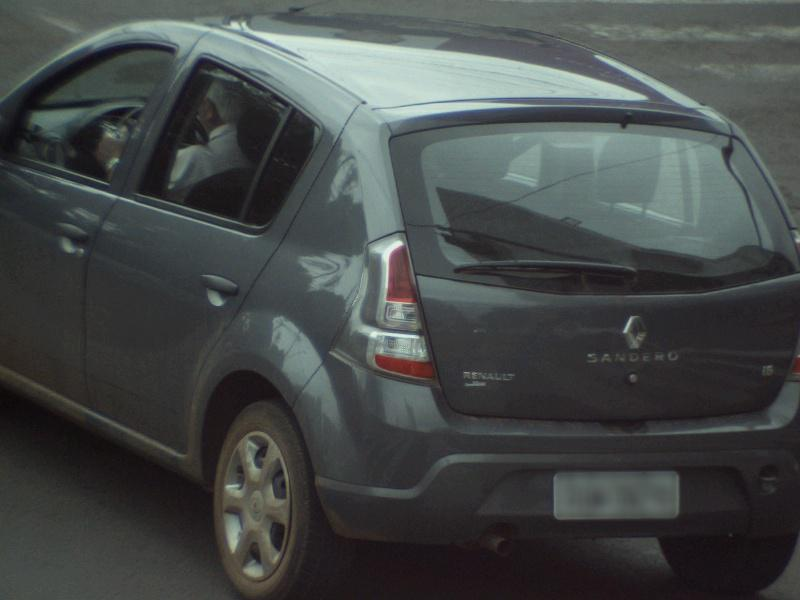
\includegraphics[width=\textwidth]{matfmaster/glava3/car.jpg}
        \caption{\textit{car}}
        \label{fig:section3_car}
    \end{subfigure}
    ~
    \begin{subfigure}[b]{0.48\textwidth}
        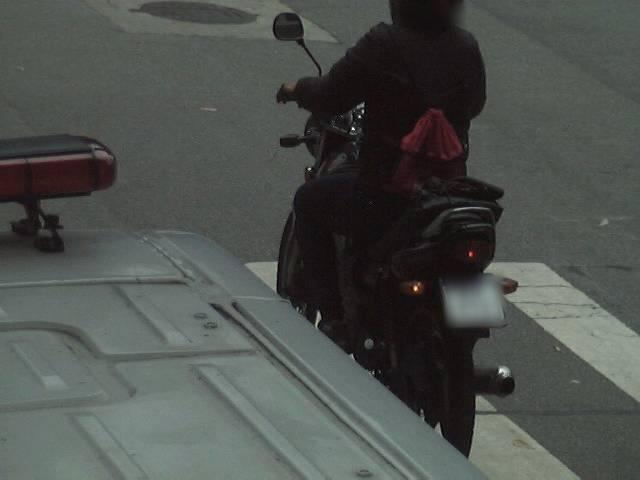
\includegraphics[width=\textwidth]{matfmaster/glava3/bike.jpg}
        \caption{\textit{motorbike}}
        \label{fig:section3_motorbike}
    \end{subfigure}
    ~
    \begin{subfigure}[b]{0.48\textwidth}
        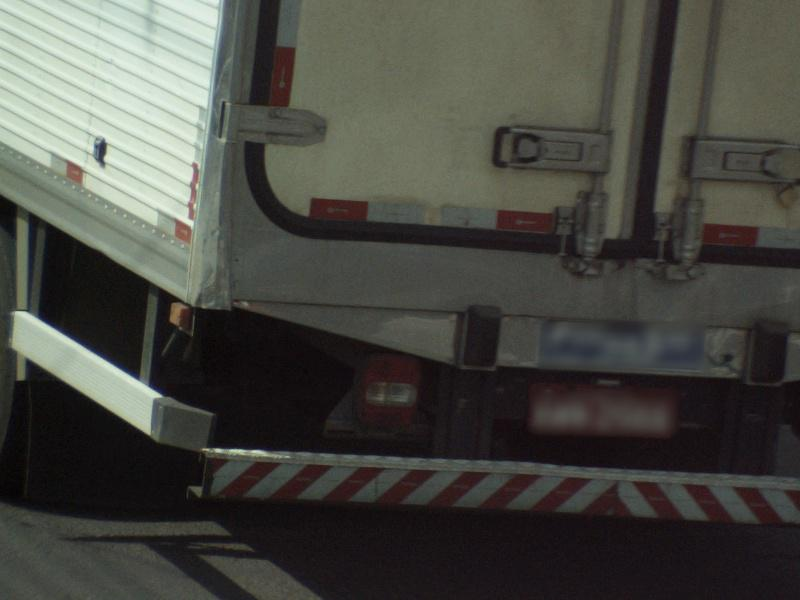
\includegraphics[width=\textwidth]{matfmaster/glava3/truck.jpg}
        \caption{\textit{truck}}
        \label{fig:section3_truck}
    \end{subfigure}
    ~
    \begin{subfigure}[b]{0.48\textwidth}
        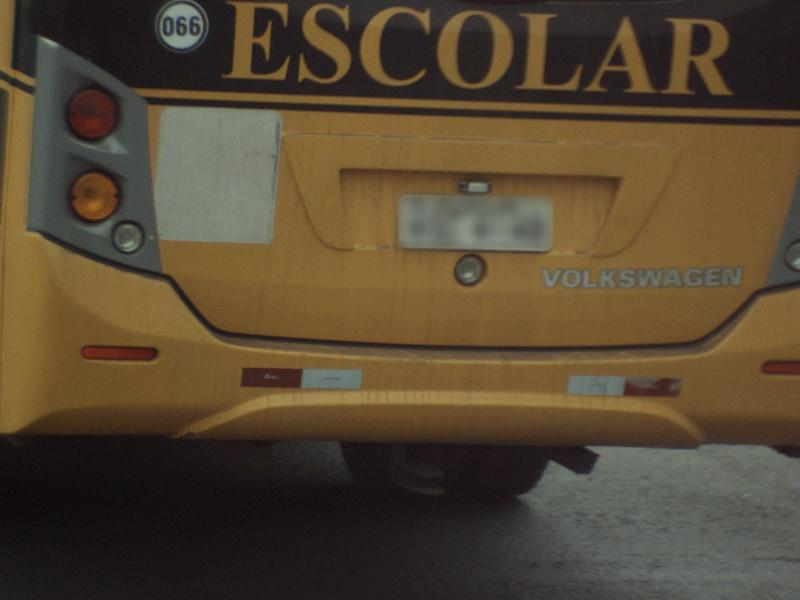
\includegraphics[width=\textwidth]{matfmaster/glava3/bus.jpg}
        \caption{\textit{bus}}
        \label{fig:section3_bus}
    \end{subfigure}
    ~
    \caption{Primeri slika iz dostupnih klasa}\label{fig:section3_allclasses}
\end{figure}


% #######################################################################
\section{Kreiranje sintetičkih podataka}
% #######################################################################

Skup za obučavanje je proširivan na dva načina: slike su generisane standardnim metodama augmentacije i modelom \textit{StyleGAN2}. U tabeli \ref{tab:section4_generisaneslike} je dat prikaz tačnog broja slika koji je generisan da bi se dobile izbalansirane klase, tačnije da svaka klasa sadrži podjednaki broj slika u skupu za obuku. 
Broj slika koji je izabran za proširivanje skupa za obuku je izabran na osnovu klase koja je sadržala najveću količinu podataka, tačnije klase \textit{motorbike}. Klasa \textit{motorbike} je proširena sa 869 slika, tačnije sa onoliko slika koliko je prisutno u skupu za obuku. Nakon proširenja skupa za obuku, svaka klasa sadrži po 1738 slika.
% Nakon proširenja skupa za obuku, klasa \textit{motorbike} je ukupno sadržala 1738 slika. Klasa \textit{truck} je proširena sa 1732, klasa \textit{bus} sa 1729  i klasa \textit{car} sa 938 slika.

\begin{table}[h!]
    \begin{center}
    \caption{Ukupan broj generisanih slika}\label{tab:section4_generisaneslike}
    \begin{tabular}{c|c|c|c|c}
        \textit{klasa} & \textit{car} &  \textit{motorbike} &  \textit{truck} & \textit{bus} \\ 
        \hline
        broj generisanih slika & 938 & 869 & 1732 & 1729 \\ 
    \end{tabular}
    \end{center}
\end{table}

% +++++++++++++++++++++++++++++++
\subsection{Generisanje podataka standardnim augmentacijama}
% +++++++++++++++++++++++++++++++

Zbog potrebe proširivanja skupa podataka \bvs, generišu se novi podaci tehnikama augmentacije (poglavlje \ref{section3_increasedata_bas}). Prošireni skup se dalje u radu naziva \bvs{standard}.
Skup augmentacija koje se primenjuju su: 
\begin{itemize}
    \item refleksija --- vrši se samo u horizontalnom smeru i vodi se računa o promeni koordinata graničnih okvira, 
    \item rotacija --- vrši sa nasumičnim uglom između jednog i pet stepeni i prazan prostor se dopunjava bojama graničnih piksela,
    \item translacija ---  pomera sliku u nasumičnom smeru za deset piksela i prazan prostor se dopunjava bojama graničnih piksela,
    \item Gausov šum --- dodaje šum na sliku sa konstantnom standardnom devijacijom 0.1 i srednjom vrednošću 1.0,
    \item Gausovo zamućenje --- primenjuje se na sliku sa konstantom standardnom devijacijom koja iznosi 7. Vrednost standardne devijacije je izabrana zbog rezolucije slika u skupu \bvs. Korišćenjem vrednosti 7 za standardnu devijaciju, slike se zamućuju dok je i dalje moguće prepoznati objekat na slici.
    \item augmentacija boja --- Parametar osvetljenja se nasumično bira iz uniformne raspodele iz intervala 0.5 do 1.5. Parametri kontrasta, intenziteta i nijanse se nasumično biraju iz uniformne raspodele iz intervala 0.0 do 10.0. Intervali augmentacija boja su izabrani nakon testiranja intervala različitih opsega. Zaključeno je da se najbolji rezultati dobijaju korišćenjem navedenih intervala.
\end{itemize}

\noindent Iz opisanog skupa augmentacija primenjuju se četiri nasumično izabrane augmentacije. Nasumično se bira jedna afina transformacija iz skupa koji čine refleksija, rotacija i translacija. Takođe, bira se jedna augmentacija između Gausovog zamućenja i Gausovog šuma. Iz skupa augmentacija boja koje čine osvetljenje, kontrast, intenzitet i nijansa, nasumično se biraju dve augmentacije. Primeri generisanih slika su prikazani na slici \ref{fig:basic_aug}.

\begin{figure}[!htbp]
\centering
  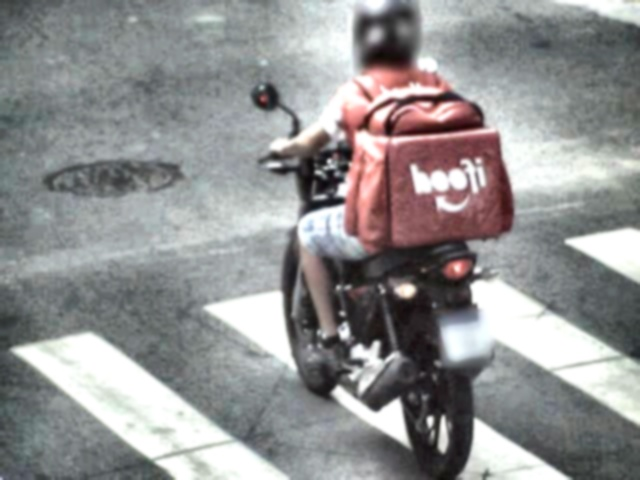
\includegraphics[width=0.32\textwidth]{matfmaster/glava4/basic_aug/1.jpg}
  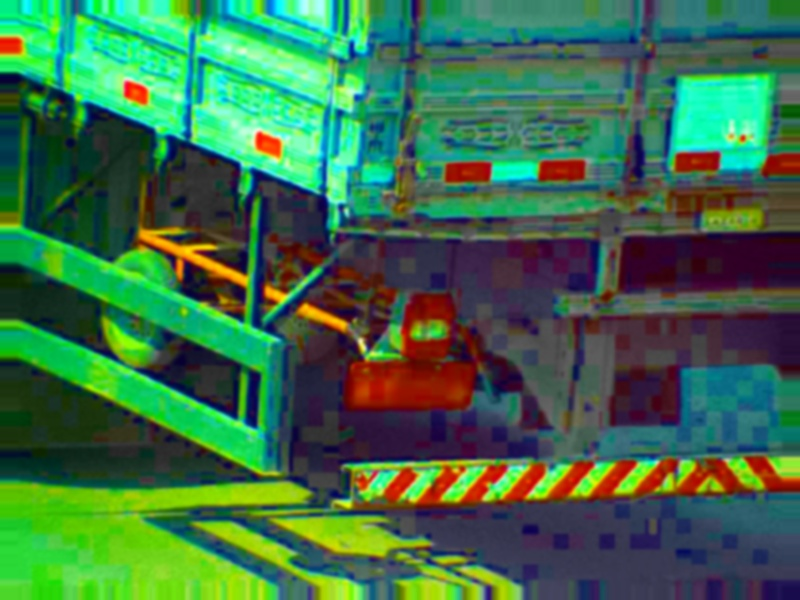
\includegraphics[width=0.32\textwidth]{matfmaster/glava4/basic_aug/2.jpg}
  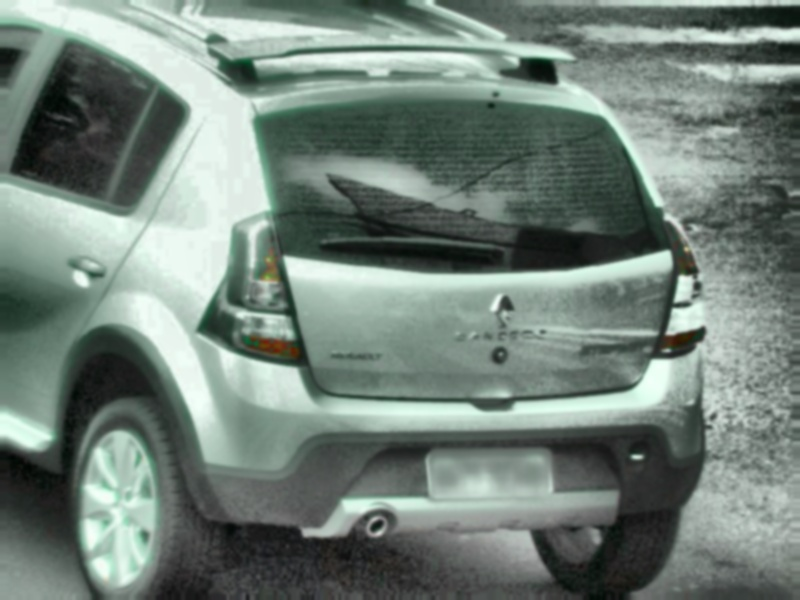
\includegraphics[width=0.32\textwidth]{matfmaster/glava4/basic_aug/3.jpg}
  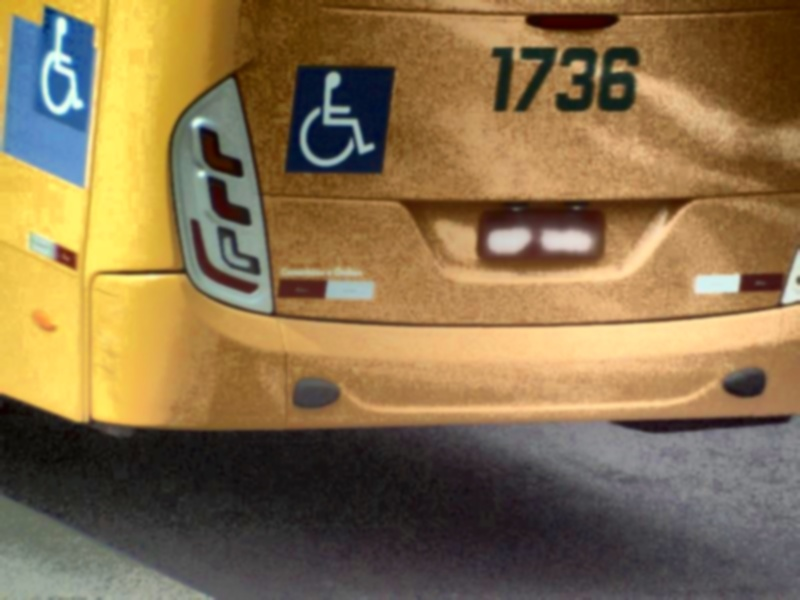
\includegraphics[width=0.32\textwidth]{matfmaster/glava4/basic_aug/4.jpg}  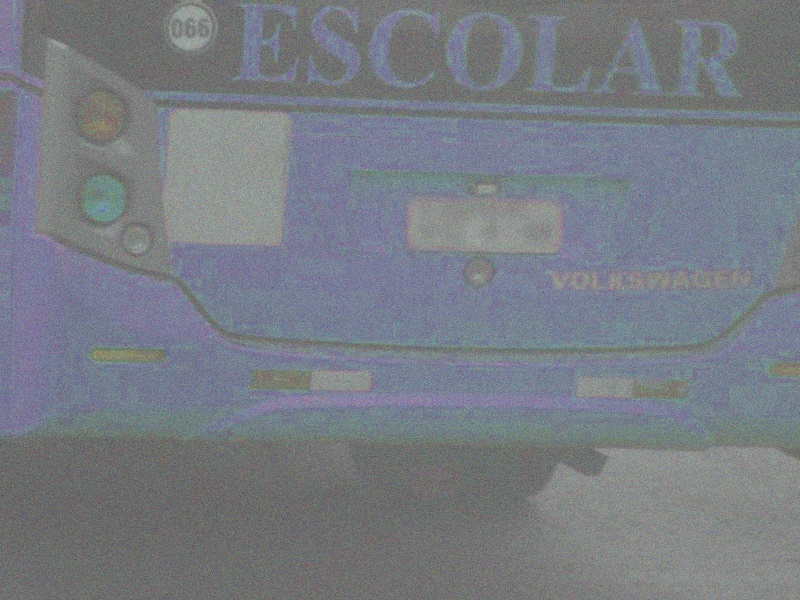
\includegraphics[width=0.32\textwidth]{matfmaster/glava4/basic_aug/5.jpg}
  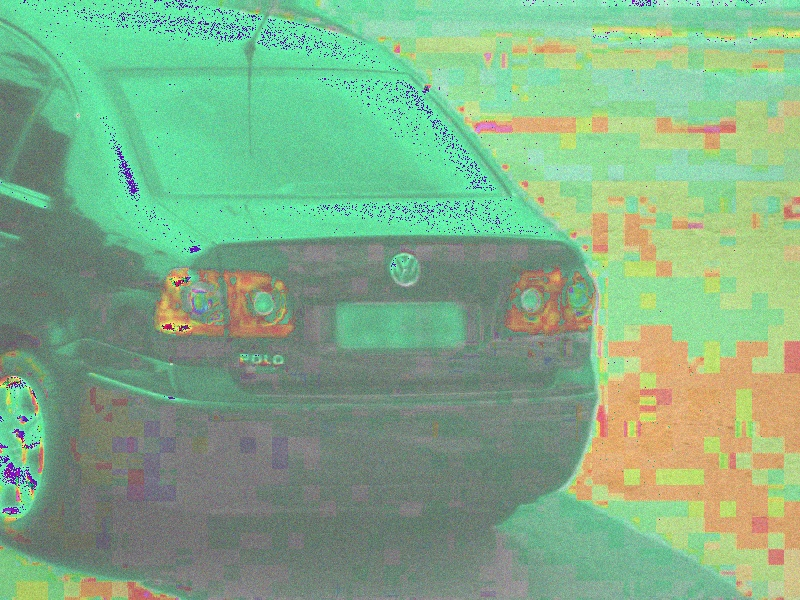
\includegraphics[width=0.32\textwidth]{matfmaster/glava4/basic_aug/6.jpg}
  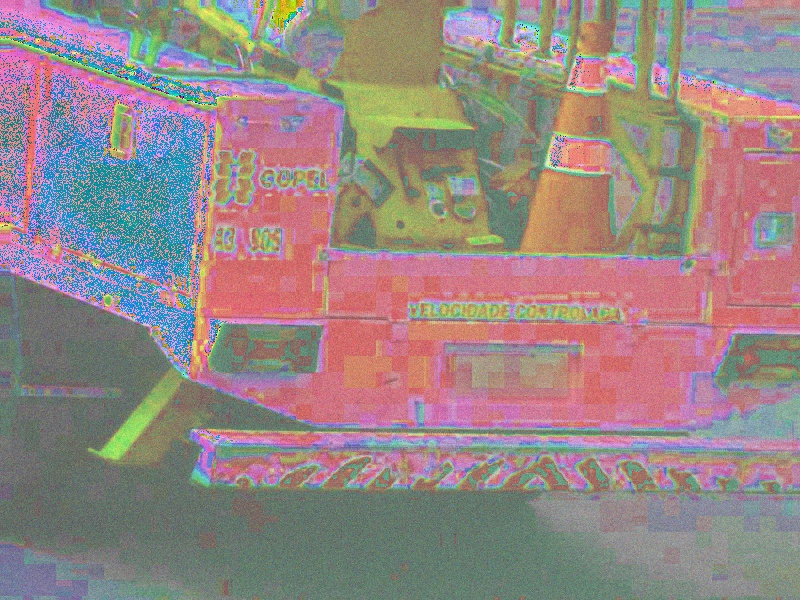
\includegraphics[width=0.32\textwidth]{matfmaster/glava4/basic_aug/7.jpg}
  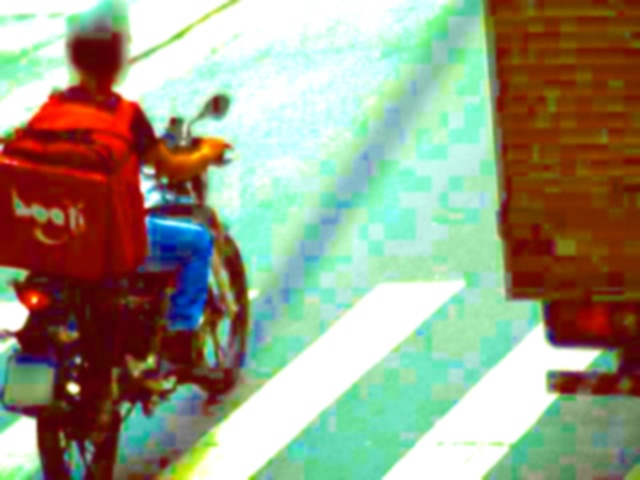
\includegraphics[width=0.32\textwidth]{matfmaster/glava4/basic_aug/8.jpg}
  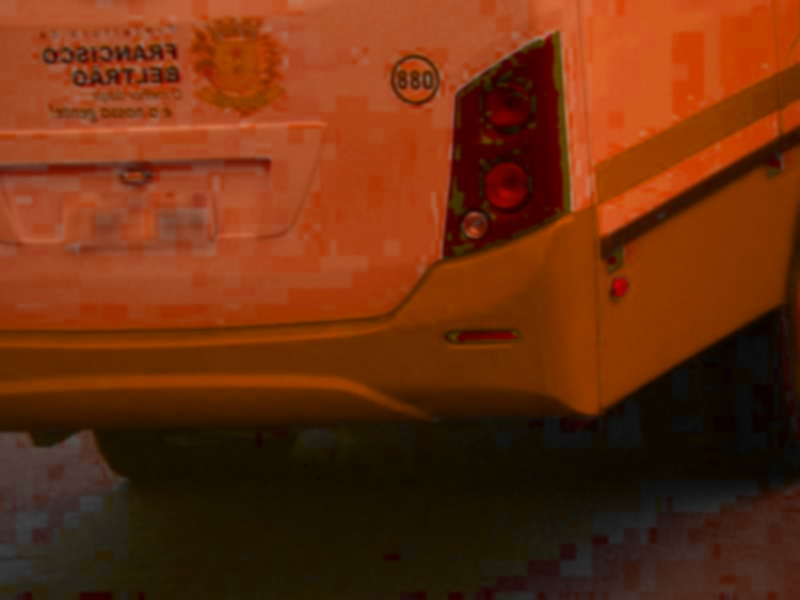
\includegraphics[width=0.32\textwidth]{matfmaster/glava4/basic_aug/9.jpg}
\caption{Primeri slika generisanih standardnim augmentacijama}\label{fig:basic_aug}
\end{figure}

  

% +++++++++++++++++++++++++++++++
\subsection{Generisanje podataka modelom \textit{StyleGAN2}}
% +++++++++++++++++++++++++++++++

Skup podataka \bvs{} se proširuje i sintetičkim podacima generisanim od strane modela \textit{StyleGAN2}. Za ovako proširen skup u radu se koristi naziv \bvs{style}. 

Međutim, problem male količine podataka se takođe javlja za generisanje novih slika modelom \textit{StyleGAN2}. Korišćenjem metode diferencijabilne augmentacije koja je navedena u poglavlju \ref{section3_increasedata_gan} prevazilazi se problem male količine podataka i model uspešno generiše slike. Implementirani metod diferencijabilne augmentacije je testiran nad skupom podataka CIFAR-10 \cite{2020diffaugment_report}.

Arhitektura modela \textit{StyleGAN2} je implementirana pomoću biblioteke \textit{Tensorflow} 2.0\footnote{Biblioteka \textit{Tensorflow} 2.0 je otvorenog koda i pruža sveobuhvatan ekosistem alata. Objavljena je 2015. godine, a objavio ju jehttps://www.overleaf.com/project/61012a88798d391d153ca901 tim \textit{Google Brain}. Osnovna namena je pravljenje modela mašinskog učenja. Biblioteka je namenjena za korišćenje u programskom jeziku \textit{Python}.}.
Generisane slike su dimenzija 512\(\times\)512. Obuka modela je trajala dvanaest do četrdeset osam sati u zavisnosti od same klase. Na svakih šest sati obuke ili, tačnije, na dvadeset pet hiljada epoha, pravljena je tačka provere (eng.~\textit{checkpoint}). Nakon svake tačke provere generisane su slike za računanje Fréchet-ove udaljenosti.

%  udaljenosti koja je procenjivala sličnost između dva skupa slika
Za evaluaciju modela \textit{StyleGAN2} koristila se metrika Fréchet-ove udaljenosti i funkcije grešaka za generativne suparničke mreže. Nakon svake tačke provere, pomoću Fréchet-ove udaljenosti procenjivana je sličnost između dva skupa slika: generisane slike pomoću modela poređene su sa pravim slikama iz validacionog skupa \bvs. Računanje Fréchet-ova udaljenosti odvijalo se na grafičkoj karti NVIDIA 780Ti i trajalo bi ukupno deset minuta. Kada se na generisanoj slici mogao prepoznati objekat i kada se funkcija greške diskriminatora i generatora nije znatno smanjivala, dalja obuka modela je prekidana. Tačan broj epoha svake klase je dat dalje u tekstu.



%___________________
\subsubsection{Klase \textit{Bus} i \textit{Truck}}
%___________________

Obuka modela \textit{StyleGAN2}-a nad klasama \textit{truck} i \textit{bus} predstavljala je veliki izazov zbog male količine dostupnih podataka. 
Rezultati Fréchet-ove udaljenosti su dati u tabelama \ref{tab:section4_fid_t}, \ref{tab:section4_fid_b}.

\begin{table}[!htb]
    \begin{minipage}{.5\linewidth}
      \caption{Klasa \textit{truck}}\label{tab:section4_fid_t}
      \centering
        \begin{tabular}{c|c}
        broj epohe &  Fréchet-ova udaljenost \\
        \hline
        25 hiljada & 432.8 \\
        \hline
        50 hiljada & 188.5 \\
        \end{tabular}
    \end{minipage}
    \begin{minipage}{.5\linewidth}
      \centering
        \caption{Klasa \textit{bus}}\label{tab:section4_fid_b}
        \begin{tabular}{c|c}
        broj epohe &  Fréchet-ova udaljenost \\
        \hline
        25 hiljada & 369.2 \\
        \hline
        50 hiljada & 220.5 \\
        \end{tabular}
    \end{minipage} 
\end{table}

Obuka modela je trajala dvadeset četiri sata. Za obuku modela je generisano dvesta hiljada slika pomoću metode diferencijabilne augmentacije. Originalan skup slika za obuku klase \textit{bus} je sadržao šest slika, a skup za obuku klase \textit{truck} je sadržao devet slika.

Iz funkcije greške (slika \ref{fig:section4_stylegan_truck_loss}) i rezultata Fréchet-ove udaljenosti (tabela \ref{tab:section4_fid_t}) za klasu \textit{truck} može se zaključiti da se daljom obukom za narednih dvadeset pet hiljada epoha ne dobijaju znatno bolji rezultati. % Bolji rezultati mogu da se postignu treniranjem za duži vremenski period, koji zahteva veće finansijske troškove. 
Primeri generisanih slika klase \textit{truck} su prikazani na slici \ref{fig:section4_stylegan_truck_images}.
Za klasu \textit{bus} iz funkcije greške (slika \ref{fig:section4_stylegan_bus_loss}) i rezultata Fréchet-ove udaljenosti (tabela \ref{tab:section4_fid_b}) može se zaključiti da se daljom obukom za narednih dvadeset pet hiljada epoha ne dobijaju znatno bolji rezultati. Primeri generisanih slika klase \textit{bus} su prikazani na slici \ref{fig:section4_stylegan_bus_images}.


\begin{figure}[!htbp]
\centering
  \includegraphics[width=0.49\textwidth]{matfmaster/stylegan/truck/g_loss.png}
  \includegraphics[width=0.49\textwidth]{matfmaster/stylegan/truck/d_loss.png}
\caption{Funkcije grešaka za klasu \textit{truck}, generator (levo) i diskriminator (desno). U oba slučaja, \textit{x} osa predstavlja epohe, dok \textit{y} osa predstavlja vrednosti odgovarajuće funkcije greške.}\label{fig:section4_stylegan_truck_loss}
\end{figure}


\begin{figure}[!htbp]
\centering
  \includegraphics[width=0.49\textwidth]{matfmaster/stylegan/bus/g_loss.png}
  \includegraphics[width=0.49\textwidth]{matfmaster/stylegan/bus/d_loss.png}
\caption{Funkcije grešaka za klasu \textit{bus}, generator (levo) i diskriminator (desno). U oba slučaja, \textit{x} osa predstavlja epohe, dok \textit{y} osa predstavlja vrednosti odgovarajuće funkcije greške.}\label{fig:section4_stylegan_bus_loss}
\end{figure}


\begin{figure}[!htbp]
\centering
    \includegraphics[width=0.49\textwidth]{matfmaster/stylegan/truck/image0.png}
    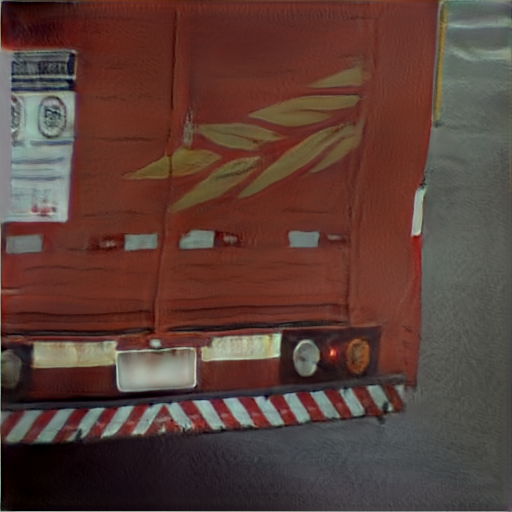
\includegraphics[width=0.49\textwidth]{matfmaster/stylegan/truck/image6.png}
\caption{Primeri generisanih slika klase \textit{truck}}
\label{fig:section4_stylegan_truck_images}
\end{figure}


\begin{figure}[!htbp]
\centering
    \includegraphics[width=0.49\textwidth]{matfmaster/stylegan/bus/image0.png}  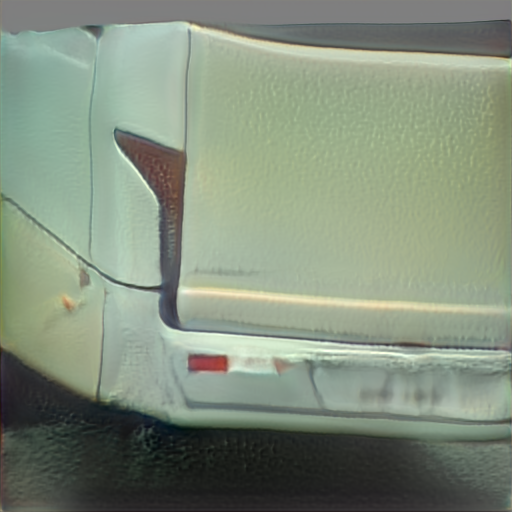
\includegraphics[width=0.49\textwidth]{matfmaster/stylegan/bus/image8.png} 
\caption{Primeri generisanih slika klase \textit{bus}}
\label{fig:section4_stylegan_bus_images}
\end{figure}

%___________________
\subsubsection{Klase \textit{car} i \textit{motorbike}}
%___________________

Obuka modela nad klasom \textit{car} je trajala oko trideset šest sati i metodom diferencijabilne augmentacije je generisano trista hiljada slika. Obuka za klasu \textit{motorbike} je trajala četrdeset osam sati i metodom diferencijabilne augmentacije je generisano četristo hiljada slika.

Za klasu \textit{car}, funkcija greške je prikazana na slici \ref{fig:section4_stylegan_car_loss}. Rezultat Fréchet-ove udaljenosti je prikazan u tabeli \ref{tab:section4_fid_c}. Daljom obukom klase \textit{car} ne dobijaju se značajna poboljšanja modela.
Primeri generisanih slika klase \textit{car} su prikazani na slici \ref{fig:section4_stylegan_car_images}.

Klasa \textit{motorbike} ima malo lošije rezultate funkcije greške koja je prikazana na slici \ref{fig:section4_stylegan_motorbike_loss}. Funkcija greške generatora raste što ukazuje da diskriminator postaje dosta bolji u prepoznavanju stvarnih od lažnih slika. Slike generisane generatorom nisu savršene, ali moguće je prepoznati glavne karakteristike objekata koji su od značaja za obuku modela detekcije objekata. Rezultat Fréchet-ove udaljenosti (tabela \ref{tab:section4_fid_m}) ukazuje da tokom obuke dolazi do poboljšanja generisanih slika. Primeri generisanih slika klase \textit{motorbike} su prikazani na slici \ref{fig:section4_stylegan_motorbike_images}.

\begin{table}[!htb]
    \begin{minipage}{.5\linewidth}
      \caption{Klasa \textit{car}}\label{tab:section4_fid_c}
      \centering
        \begin{tabular}{c|c}
        broj epohe &  Fréchet-ova udaljenost \\
        \hline
        25 hiljada & 107.6 \\
        \hline
        75 hiljada & 87.5 \\
        \end{tabular}
    \end{minipage}%
    \begin{minipage}{.5\linewidth}
      \centering
        \caption{Klasa \textit{motorbike}}\label{tab:section4_fid_m}
        \begin{tabular}{c|c}
        broj epohe &  Fréchet-ova udaljenost \\
        \hline
        25 hiljada & 386.8 \\
        \hline
        100 hiljada & 151.1 \\
        \end{tabular}
    \end{minipage} 
\end{table}


\begin{figure}[!htbp]
\centering
  \includegraphics[width=0.49\textwidth]{matfmaster/stylegan/car/g_loss.png}
  \includegraphics[width=0.49\textwidth]{matfmaster/stylegan/car/d_loss.png}
\caption{Funkcije grešaka za klasu \textit{car}, generator (levo) i diskriminator (desno). U oba slučaja, \textit{x} osa predstavlja epohe, dok \textit{y} osa predstavlja vrednosti odgovarajuće funkcije greške.}\label{fig:section4_stylegan_car_loss}
\end{figure}

\begin{figure}[!htbp]
\centering
  \includegraphics[width=0.49\textwidth]{matfmaster/stylegan/motorbike/g_loss.png}
  \includegraphics[width=0.49\textwidth]{matfmaster/stylegan/motorbike/d_loss.png}
\caption{Funkcije grešaka za klasu \textit{motorbike}, generator (levo) i diskriminator (desno). U oba slučaja, \textit{x} osa predstavlja epohe, dok \textit{y} osa predstavlja vrednosti odgovarajuće funkcije greške. }\label{fig:section4_stylegan_motorbike_loss}
\end{figure}

\begin{figure}[!htbp]
\centering
    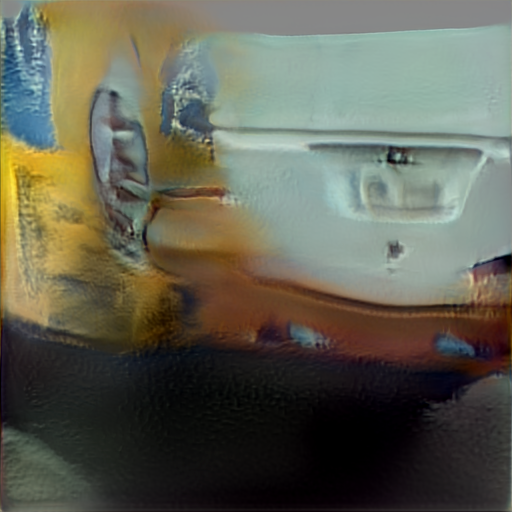
\includegraphics[width=0.49\textwidth]{matfmaster/stylegan/car/image1.png}  \includegraphics[width=0.49\textwidth]{matfmaster/stylegan/car/image2.png}
\caption{Primeri generisanih slika klase \textit{car}}
\label{fig:section4_stylegan_car_images}
\end{figure}

\begin{figure}[!htbp]
\centering
    \includegraphics[width=0.49\textwidth]{matfmaster/stylegan/motorbike/image2.png}
    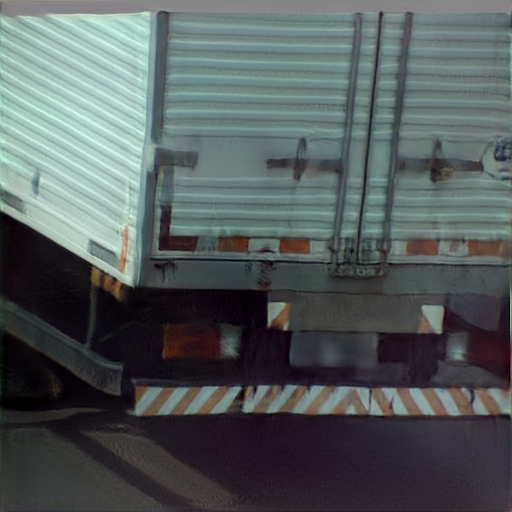
\includegraphics[width=0.49\textwidth]{matfmaster/stylegan/motorbike/image9.png}
\caption{Primeri generisanih slika klase \textit{motoribke}}
\label{fig:section4_stylegan_motorbike_images}
\end{figure}

Generisane slike nisu savršene, ali je moguće prepoznati glavne karakteristike objekata. Neke generisane slike su sklone da sadrže artifakte i zamućenosti.% ali se one uzimaju kao dodatna vrsta regularizacije.


% #######################################################################
% \clearpage
\section{Model za detekciju i predviđanje objekata VGG16}
% #######################################################################

Osnovni model VGG16 je ograničen na klasifikaciju slika bez predviđanja graničnih okvira i u okviru ovog rada osnovni model je proširen odgovarajućim mrežama da se omogući predviđanje graničnih okvira. Osnovni model je proširen na sledeći način:
\begin{itemize}
\item Na poslednji sloj dodato je račvanje na dve nove duboko povezane mreže dubine četiri.
\item Na izlazu prve mreže dodata je aktivaciona funkcija \textit{softmax}, koja se tumači kao dodeljivanje verovatnoće da objekat pripada jednoj od četiri klase.
\item Na izlazu druge mreže dodata je \textit{sigmoid}-na aktivaciona funkcija, koja se tumači kao dodeljivanje relativnih graničnih okvira predviđenim objektima.
\end{itemize}
Prošireni osnovni model je obučen na skupu podataka \bvs{} u trajanju od oko deset minuta.

Zbog problema neizbalansiranosti klasa koji se javlja u skupu podataka \bvs, dobija se rezultat modela koji ima visoku pristrasnost ka klasi \textit{car}, kao što se vidi iz tabele \ref{tab:section4_vgg16_confusionmatrix}. Model pogrešno daje izlaze graničnih okvira, kao što je prikazano na slici \ref{fig:section4_vgg16prediction}.

Rezultati evaluacije modela su dati u tabeli \ref{tab:section4_vgg16_results}. Iz rezultata se vidi da se model ponaša loše nad celim skupom podataka. Neki od razloga koji utiču da model daje loše rezultate je visoka neizbalansiranost između klasa, mala količina dostupnih podataka i model je suviše jednostavan i ne može da obradi sve moguće karakteristike koje se nalaze na slikama. Preciznost klasa u odnosu na IoU prag je prikazana na slici \ref{fig:section4_vgg16_prc}.

Kako je osnovni model VGG16 proširen, ne postoje slobodno dostupne odgovarajuće težine drugog modela koje mogu da se koriste za metodu transfernog učenja. Korišćenjem proširenog skupa podataka \bvs{standard} ili \bvs{style}, dostupna količina podataka bi i dalje bila nedovoljna. Za obuku modela potrebno je desetine hiljada slika koje ni u proširenim skupovima \bvs{} nisu dostupne.

% Matricja konfuzije
\begin{table}[h!]
    \begin{center}
    \caption{Matrica konfuzije modela VGG16 za IoU prag 0.5 i prag ocene pouzdanosti za prepoznatu klasu 0.5}
    \begin{tabular}{ l|c|c|c|c|c|}
                  & car  & motorbike & bus & truck & bez detekcije \\ \hline
    car           & 85   & 26        & 0   & 1     & 0             \\ 
    motorbike     & 0    & 0         & 0   & 0     & 0             \\ 
    bus           & 0    & 0         & 0   & 0     & 0             \\ 
    truck         & 0    & 0         & 0   & 0     & 0             \\ 
    bez detekcije & 4    & 71        & 1   & 0     & 0             \\ \hline
    \hline
    \end{tabular}
    \label{tab:section4_vgg16_confusionmatrix}
    \end{center}
\end{table}


% Tabela sa rezultatima, preurediti 
\begin{table}[h!]
    \begin{center}
    \caption{Rezultati modela VGG16}
    \begin{tabular}{|m{10em}|c|c|}
        \toprule
        klasa     & prosečna preciznost (jedn.~\ref{eq:ap}) & srednja $F_1$-mera (jedn.~\ref{eq:f1a})  \\ \hline
        \midrule
        car       & 0.95  & 0.57 \\ \hline
        motorbike & 0.0   & 0.0 \\ \hline
        bus       & 0.0   & 0.0 \\ \hline
        truck     & 0.0   & 0.0 \\ \hline
        \bottomrule
        Srednja prosečna preciznost (jedn.~\ref{eq:map}) & \multicolumn{2}{c|}{0.24}  \\ \hline
        Srednja težinska $F_1$-mera (jedn.~\ref{eq:f1wa}) & \multicolumn{2}{c|}{0.27}  \\ \hline
    \end{tabular}
    \label{tab:section4_vgg16_results}
    \end{center}
\end{table}

% CUrve graph
\begin{figure}[!ht]
    \centering
    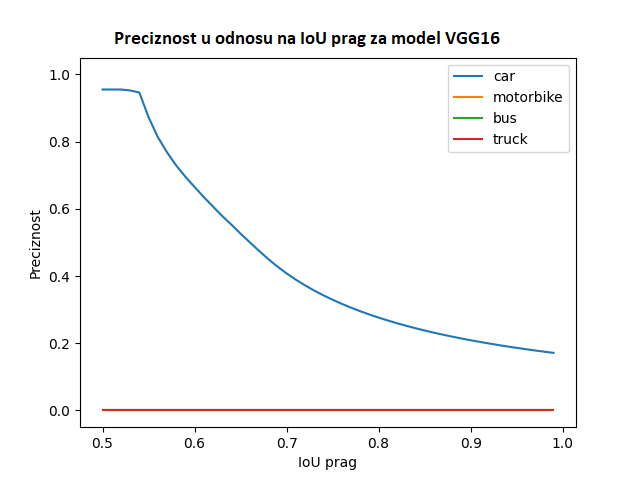
\includegraphics[width=1\textwidth]{matfmaster/glava4/precision_vs_iou_threshold_VGG16.png}
    \caption{Preciznost u odnosu na IoU prag za model VGG16. Za klase \textit{motorbike}, \textit{bus} i \textit{truck} preciznost u svim vrednostima IoU iznosi 0.}
    \label{fig:section4_vgg16_prc}
\end{figure}

% Slike klasa
\begin{figure}
    \centering
    \begin{subfigure}[b]{0.35\textwidth}
        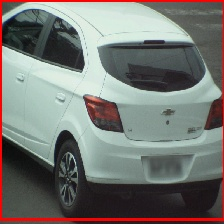
\includegraphics[width=\textwidth]{matfmaster/vgg16_base/car_real.jpg}
        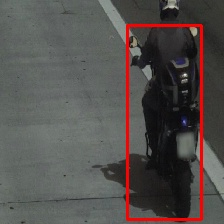
\includegraphics[width=\textwidth]{matfmaster/vgg16_base/motorbike_real.jpg}
        \includegraphics[width=\textwidth]{matfmaster/vgg16_base/bus_real.jpg}
        \includegraphics[width=\textwidth]{matfmaster/vgg16_base/truck_real.jpg}
        \caption{Stvarni okviri}
    \end{subfigure}
    ~
    \begin{subfigure}[b]{0.35\textwidth}
        \includegraphics[width=\textwidth]{matfmaster/vgg16_base/car_pred.jpg}
        \includegraphics[width=\textwidth]{matfmaster/vgg16_base/motorbike_pred.jpg}
        \includegraphics[width=\textwidth]{matfmaster/vgg16_base/bus_pred.jpg}
        \includegraphics[width=\textwidth]{matfmaster/vgg16_base/truck_pred.jpg}
        \caption{Predviđeni okviri}
    \end{subfigure}
    ~
    \caption{Primeri rezultata modela VGG16 nad validacionim skupom podataka}
    \label{fig:section4_vgg16prediction}
\end{figure}



% #######################################################################
% \clearpage
\section{Model za detekciju i predviđanje objekata YOLO}
% #######################################################################

Kako model VGG16 ne može da d\^{a} zadovoljavajuće rezultate, u okviru rada razmatra se i model za detekciju i predviđanje objekata YOLO. Koriste se dve konfiguracije modela YOLO. Prva konfiguracija modela YOLO služi za poređenje rezultata, i u mogućnosti je da predvidi do osamdeset klasa. Prva konfiguracija je prilagođena za skup podataka COCO (eng.~\textit{common objects in context}). Druga konfiguracija modela YOLO je u stanju da predvidi do četiri klase i prilagođena je za skup podataka \bvs.


% +++++++++++++++++++++++++++++++
\subsection{Predikcija modela YOLO koji je obučen na skupu podataka COCO}
% +++++++++++++++++++++++++++++++

Koristi se model YOLO koji je obučen na skupu podataka COCO koji sadrži osamdeset klasa i 328 hiljada slika. Dalje u radu model YOLO obučen na skupu podataka COCO se označava sa $\yolo_{coco}$. Evaluacija modela se vrši nad validacionim skupom podataka \bvs. Matrica konfuzije je izračunata za vrednost IoU praga 0.5 i za ocenu pouzdanosti veću od 0.5. Tokom računanja prosečne preciznosti i srednje $F_1$-mere nije se uzimala u obzir ocena pouzdanosti klasa. 

Iz rezultata matrice konfuzije (tabela \ref{tab:section4_yolo4base_confusionmatrix}) i metoda evaluacije modela (tabela \ref{tab:section4_yolo4base_results}) zaključuje se sledeće:
\begin{itemize}
    \item Klasu \textit{car} model $\yolo_{coco}$ predviđa sa visokom ocenom preciznosti. Predviđena je osamdeset i jedna instanca od ukupno osamdeset i devet. Iz matrice konfuzije može da se vidi da je model $\yolo_{coco}$ za tri instance imao ocenu pouzdanosti manju od 0.5. Takođe, pogrešno se klasifikuje pet instanci kao instance klase \textit{truck}. Prosečna preciznost za klasu \textit{car} iznosi 0.88, dok srednja $F_1$-mera iznosi 0.91.
    \item Klasa \textit{motorbike} se predviđa lošije od klase \textit{car}. Model $\yolo_{coco}$ predviđa trideset sedam od ukupno devedeset sedam instanci. Većina instanci, tačnije četrdeset devet, za ocenu pouzdanosti ima vrednost manju od 0.5. Ocene pouzdanosti klase ukazuju da model nije siguran pri predviđanju instanci iz klase \textit{motorbike}. Prosečna preciznost iznosi 0.77 i srednja $F_1$-mera iznosi 0.48.
    \item Klasa \textit{bus} sadrži jednu sliku za validaciju i ona se ne predviđa modelom $\yolo_{coco}$. Prosečna preciznost i srednja $F_1$-mera iznose 0.
    \item Klasa \textit{truck} se uspešno predviđa modelom $\yolo_{coco}$. Prosečna preciznost iznosi 1.0 i srednja $F_1$-mera iznosi 0.99.
\end{itemize}

Preciznost klasa u odnosu na IoU prag je prikazana na slici \ref{fig:section4_yolo4base_prc}. Model $\yolo_{coco}$ ima srednju prosečnu preciznost (mAP) koja iznosi 0.66 i srednju težinsku $F_1$-meru koja iznosi 0.69. Kod predviđanja modela $\yolo_{coco}$ možemo da zaključimo da dobro prepoznaje objekte klase \textit{car} i \textit{truck}. Problem koji se uočava kod predviđanja tih klasa je da postoje objekti koji imaju slične karakteristike. Takav problem se može uočiti na slici \ref{fig:section4_yolo4base_problemimages}. Model $\yolo_{coco}$ je uspešno klasifikovao 40\% instanci klase \textit{motorbike} iz validacionog skupa \bvs. Instanca klase \textit{bus} se ne klasifikuje ispravno modelom  $\yolo_{coco}$.

Na slici \ref{fig:section4_yolo4base_images} su prikazana neka predviđanja modela $\yolo_{coco}$. Slika prikazuje da su se uspešno detektovali neki od objekata koji pripadaju klasama \textit{car} (gore desno), \textit{motorbike} (sredina desno) i \textit{truck} (dole levo). Na slici koja pripada klasi \textit{motorbike} (sredina levo), uočavamo da je model uspešno detektovao čoveka, ali nije uspeo da detektuje objekat klase \textit{motorbike}, odnosno ocena pouzdanosti je bila veoma mala, tj. iznosila je 0.2. 

% Matricja konfuzije
\begin{table}
    \begin{center}
    \caption{Matrica konfuzije modela $\yolo_{coco}$ za IoU prag 0.5 i prag ocene pouzdanosti za prepoznatu klasu veći od 0.5 }
    \begin{tabular}{ l|c|c|c|c|c|}
                  & car  & motorbike & bus & truck & bez detekcije \\ \hline
    car           & 81   & 0         & 0   & 0     & 0             \\ 
    motorbike     & 0    & 37        & 0   & 0     & 0             \\ 
    bus           & 0    & 0         & 0   & 0     & 0             \\ 
    truck         & 5    & 0         & 0   & 1     & 0             \\ 
    bez detekcije & 3    & 52        & 1   & 0     & 0             \\ \hline
    \hline
    \end{tabular}
    \label{tab:section4_yolo4base_confusionmatrix}
    \end{center}
\end{table}


% Tabela sa rezultatima
\begin{table}
    \begin{center}
    \caption{Rezultati evaluacije modela $\yolo_{coco}$}
        \begin{tabular}{|m{10em}|c|c|}
        \toprule
        klasa     & prosečna preciznost (jedn.~\ref{eq:ap}) & srednja $F_1$-mera (jedn.~\ref{eq:f1a})  \\ \hline
        \midrule
        car       & 0.88  & 0.91 \\ \hline
        motorbike & 0.77  & 0.48 \\ \hline
        bus       & 0.0   & 0.0  \\ \hline
        truck     & 1.0   & 0.99 \\ \hline
        \bottomrule
        Srednja prosečna preciznost (jedn.~\ref{eq:map}) & \multicolumn{2}{c|}{0.66}  \\ \hline
        Srednja težinska $F_1$-mera (jedn.~\ref{eq:f1wa}) & \multicolumn{2}{c|}{0.69}  \\ \hline
    \end{tabular}
    \label{tab:section4_yolo4base_results}
    \end{center}
\end{table}


% kriva IOU i Preciznost
\begin{figure}[!ht]
    \centering
    \includegraphics[width=1\textwidth]{matfmaster/glava4/precision_vs_iou_threshold_yolo4.png}
    \caption{Preciznost u odnosu na IoU prag [0.5,1) modela $\yolo_{coco}$}
    \label{fig:section4_yolo4base_prc}
\end{figure}


\begin{figure}[htbp]
    \centering
      \includegraphics[width=0.49\textwidth]{matfmaster/yolo/v4/base/car_0.jpg}
      \includegraphics[width=0.49\textwidth]{matfmaster/yolo/v4/base/car_1.jpg}
      \includegraphics[width=0.49\textwidth]{matfmaster/yolo/v4/base/motorbike_0.jpg}
      \includegraphics[width=0.49\textwidth]{matfmaster/yolo/v4/base/motorbike_1.jpg}
      \includegraphics[width=0.49\textwidth]{matfmaster/yolo/v4/base/truck_0.jpg}
      \includegraphics[width=0.49\textwidth]{matfmaster/yolo/v4/base/bus_0.jpg}
    \caption{Slike iz validacionog skupa i predviđanja nad njima modelom $\yolo_{coco}$, klasa \textit{car} (gore), klasa \textit{motorbike} (sredina),  klasa \textit{truck} (dole levo) i  klasa \textit{bus} (dole desno). Objekti na slikama bez graničnih okvira nisu uspešno detektovani.} \label{fig:section4_yolo4base_images}
\end{figure}

\begin{figure}[htbp]
    \centering
      \includegraphics[width=0.49\textwidth]{matfmaster/glava4/carproblem.jpg}
      \includegraphics[width=0.49\textwidth]{matfmaster/glava4/truckproblem.jpg}
    \caption{Slične karakteristike dveju različitih klasa, klasa \textit{car} (levo) i klasa \textit{truck} (desno) } \label{fig:section4_yolo4base_problemimages}
\end{figure}


% +++++++++++++++++++++++++++++++
% \clearpage
\subsection{Obuka modela pomoću tehinke transfernog učenja}
% +++++++++++++++++++++++++++++++
Radi poboljšanja rezultata, naredni modeli su obučeni koristeći težine modela obučene na skupu podataka COCO. Kako postoji razlika u broju klasa između skupa podataka BVS i COCO skupa, neki delovi težina su odbačeni.

Modeli su obučeni na slikama rezolucije do 512$\times$512. Slikama je nasumično menjana veličina iz intervala 224$\times$224 do 512$\times$512, sa korakom 32$\times$32. Obuka modela je bila ograničena na sto deset epoha. U prvih deset epoha obuka modela je vršena u samo poslednja tri sloja, dok su ostali slojevi bili zamrznuti. Nakon deset epoha, odmrznuti su ostali slojevi i nastavljeno je sa normalnom obukom modela. U prvih deset epoha, stopa obuke optimizatora modela se umanjivala svake tri epohe za konstantu vrednost 0.001, u slučaju da se funkcija greške nije smanjivala. Nakon deset epoha stopa obuke optimizatora modela se umanjivala za 0.00001. Time se postizalo usavršavanje modela. Takođe, postavljena je zastavica za rano zaustavljanje ukoliko se u deset uzastopnih epoha funkcija greške nije umanjila.


%_______________________________________________________________________________________
\subsubsection{Obuka modela pomoću tehnike transfernog učenja na skupu podataka BVS}
%_______________________________________________________________________________________
Koristi se model YOLO koji je obučen na skupu podataka \bvs{} koji sadrži četiri klase i 1872 slike. Dalje u radu model YOLO obučen na skupu podataka \bvs{} se označava sa $\yolo_{\bvs}$. Funkcija greške modela je prikazana na slici \ref{fig:section4_yolo4noaug_loss}. Iz funkcije greške se vidi da je došlo do ranog zaustavljanja obuke modela nakon dvadeset sedam epoha. Obuka modela je trajala oko dva sata.
%Model je obučen na grafičkoj karti NVIDIA Tesla P100-PCIE  u trajanju od oko dva sata.

% Funkcija greške
\begin{figure}[!ht]
\centering
  \includegraphics[width=0.90\textwidth]{matfmaster/yolo/v4/without_augmentation/epoch_loss.png}
\caption{Funkcija greške $\yolo_{\bvs}$ modela}
\label{fig:section4_yolo4noaug_loss}
\end{figure}

Iz rezultata matrice konfuzije (tabela \ref{tab:section4_yolo4noaug_confusionmatrix}) i metoda evaluacije modela (tabela \ref{tab:section4_yolo4noaug_results}) zaključuje se sledeće:
\begin{itemize}
    \item klasu \textit{car} model $\yolo_{\bvs}$ uspešno klasifikuje u 66\% slučajeva. Predviđeno je pedest devet od ukupno osamdeset devet instanci. Iz matrice konfuzije može da se vidi da je model $\yolo_{\bvs}$ za trideset instanci ima ocenu pouzdanosti manju od 0.5.  Prosečna preciznost za klasu \textit{car} iznosi 0.06 i srednja $F_1$-mera iznosi 0.04, što ukazuje na veoma loše rezultate.
    \item deset instanci klase \textit{motorbike} se pogrešno predviđa. Model $\yolo_{\bvs}$ ih  predvideo kao instance klase \textit{car}. Ostatak klase \textit{motorbike} se ne predviđa. Prosečna preciznost i srednja $F_1$-mera iznose 0.
    \item klasa \textit{bus} i klasa \textit{truck} se ne predviđaju ni u jednoj instanci. Prosečna preciznost i srednja $F_1$-mera takođe iznose 0.
\end{itemize}

% Matricja konfuzije
\begin{table}
    \begin{center}
    \caption{Matrica konfuzije modela $\yolo_{bvs}$ za IoU prag 0.5 i prag ocene pouzdanosti za prepoznatu klasu 0.5 }
    \begin{tabular}{ l|c|c|c|c|c|}
                  & car  & motorbike & bus & truck & bez detekcije \\ \hline
    car           & 59   & 10        & 0   & 0     & 0             \\ 
    motorbike     & 0    & 0         & 0   & 0     & 0             \\ 
    bus           & 0    & 0         & 0   & 0     & 0             \\ 
    truck         & 0    & 0         & 0   & 0     & 0             \\ 
    bez detekcije & 30   & 79        & 1   & 1     & 0             \\ \hline
    \end{tabular}
    \label{tab:section4_yolo4noaug_confusionmatrix}
    \end{center}
\end{table}

% Tabela sa rezultatima
\begin{table}
    \begin{center}
    \caption{Rezultati evaluacije modela $\yolo_{bvs}$}
        \begin{tabular}{|m{10em}|c|c|}
        \toprule
        klasa     & prosečna preciznost (jedn.~\ref{eq:ap}) & srednja $F_1$-mera (jedn.~\ref{eq:f1a})  \\ \hline
        \midrule
        car       & 0.06  & 0.04 \\ \hline
        motorbike & 0.00  & 0.00 \\ \hline
        bus       & 0.00  & 0.00 \\ \hline
        truck     & 0.00  & 0.00 \\ \hline
        \bottomrule
        Srednja prosečna preciznost (jedn.~\ref{eq:map}) & \multicolumn{2}{c|}{0.01}  \\ \hline
        Srednja težinska $F_1$-mera (jedn.~\ref{eq:f1wa}) & \multicolumn{2}{c|}{0.02}  \\ \hline
    \end{tabular}
    \label{tab:section4_yolo4noaug_results}
    \end{center}
\end{table}

Preciznost klasa u odnosu na IoU prag je prikazana na slici \ref{fig:section4_yolo4noaug_prc}. Model $\yolo_{bvs}$ ima srednju prosečnu preciznost (mAP) koja iznosi 0.01 i srednju težinsku $F_1$-meru koja iznosi 0.02. Može se zaključiti bez dalje analize da se model ponaša loše i da su predviđanja loša. Primer rezultata detekcije je prikazan na slici \ref{fig:section4_yolo4noaug_images}. Sa slika se vidi da model klasifikuje samo klasu \textit{car} i to veoma loše sa velikim brojem graničnih okvira.

% kriva IOU i Preciznost
\begin{figure}[!ht]
    \centering
    \includegraphics[width=1\textwidth]{matfmaster/glava4/precision_vs_iou_threshold_NOaugment.png}
    \caption{Preciznost u odnosu na IoU prag [0.5,1) modela $\yolo_{\bvs}$, za klase \textit{motorbike}, \textit{bus} i \textit{truck} preciznost u svim vrednostima IoU iznosi 0}
    \label{fig:section4_yolo4noaug_prc}
\end{figure}


\begin{figure}[!htbp]
\centering
  \includegraphics[width=0.49\textwidth]{matfmaster/yolo/v4/without_augmentation/car_0f.jpg}
  \includegraphics[width=0.49\textwidth]{matfmaster/yolo/v4/without_augmentation/car_1f.jpg}
  \includegraphics[width=0.49\textwidth]{matfmaster/yolo/v4/without_augmentation/motorbike_0f.jpg}
  \includegraphics[width=0.49\textwidth]{matfmaster/yolo/v4/without_augmentation/motorbike_1f.jpg}
  \includegraphics[width=0.49\textwidth]{matfmaster/yolo/v4/without_augmentation/truck_0f.jpg}
  \includegraphics[width=0.49\textwidth]{matfmaster/yolo/v4/without_augmentation/bus_0f.jpg}
\caption{Slike iz validacionog skupa i predviđanja nad njima modelom $\yolo_{\bvs}$, klasa \textit{car} (gore), klasa \textit{motorbike} (sredina), klasa \textit{truck} (dole levo) i klasa \textit{bus} (dole desno). Objekti na slikama bez graničnih okvira nisu uspešno detektovani.}
\label{fig:section4_yolo4noaug_images}
\end{figure}



%_______________________________________________________________________________________
% \clearpage
\subsubsection{Obuka modela pomoću tehnike transfernog učenja na skupu podataka \bvs{standard}}
%_______________________________________________________________________________________

Koristi se model YOLO koji je obučen na skupu podataka \bvs{standard} koji sadrži četiri klase i 6952 slike. Dalje u radu model YOLO obučen na skupu podataka \bvs{standard} se označava sa $\yolo_{\bvs{standard}}$. Funkcija greške modela je prikazana na slici \ref{fig:section4_yolov4baseaug_loss}. Iz funkcije greške se vidi da je došlo do ranog zaustavljanja obuke modela nakon četrdeset epoha. Obuka modela je trajala jedanaest sati.
%Model je obučen na NVIDIA Tesla P100-PCIE grafičkoj karti u trajanju od jedanaest sati.

% Funkcija greške
\begin{figure}[!htbp]
\centering
  \includegraphics[width=0.70\textwidth]{matfmaster/yolo/v4/basic_augmentation/epoch_loss.png}
\caption{Funkcija greške  $\yolo_{\bvs{standard}}$ modela}
\label{fig:section4_yolov4baseaug_loss}
\end{figure}

Iz rezultata matrice konfuzije (tabela \ref{tab:section4_yolo4baseaug_confusionmatrix}) i metoda evaluacije modela (tabela \ref{tab:section4_yolo4baseaug_results}) zaključuje se sledeće:
\begin{itemize}
    \item klasu \textit{car} model  $\yolo_{\bvs{standard}}$ predviđa sa visokom ocenom preciznosti. Predviđeno je osamdeset dva od ukupno osamdeset devet instanci. Iz matrice konfuzije može da se vidi da je model  $\yolo_{\bvs{standard}}$ za sedam instanci imao ocenu pouzdanosti manju od 0.5. Prosečna preciznost za klasu \textit{car} iznosi 1.0\footnote{Za računanje prosečne preciznosti i srednje $F_1$-mere nije se koristila ocena pouzdanosti, već samo da li je objekat uspešno klasifikovan ili ne.}, dok srednja $F_1$-mera iznosi 0.92. Ovi rezultati ukazuju na veoma dobro predviđanje modela  $\yolo_{\bvs{standard}}$ nad klasom \textit{car}.
    \item klasa \textit{motorbike} se predviđa bolje od klase \textit{car}. Model  $\yolo_{\bvs{standard}}$ predviđa devedeset pet od ukupno devedeset sedam instanci. Dve instance za ocenu pouzdanosti imaju vrednost manju od 0.5. Prosečna preciznost iznosi 0.99 i srednja $F_1$-mera iznosi 0.97.
    \item klasa \textit{truck} se pogrešno predviđa kao klasa \textit{car}. 
    \item  klasa \textit{bus} se ne predviđa modelom  $\yolo_{\bvs{standard}}$.
\end{itemize}


% Matricja konfuzije
\begin{table}
    \begin{center}
    \caption{Matrica konfuzije modela $\yolo_{\bvs{standard}}$ za IoU prag 0.5 i prag pozdanosti za prepoznatu klasu 0.5 }
    \begin{tabular}{ l|c|c|c|c|c|}
                  & car  & motorbike & bus & truck & bez detekcije \\ \hline
    car           & 82   & 0         & 0   & 1     & 0             \\ 
    motorbike     & 0    & 95        & 0   & 0     & 0             \\ 
    bus           & 0    & 0         & 0   & 0     & 0             \\ 
    truck         & 0    & 0         & 0   & 0     & 0             \\ 
    bez detekcije & 7    & 2         & 1   & 0     & 0             \\ \hline
    \hline
    \end{tabular}
    \label{tab:section4_yolo4baseaug_confusionmatrix}
    \end{center}
\end{table}


% Tabela sa rezultatima
\begin{table}
    \begin{center}
    \caption{Rezultati modela $\yolo_{\bvs{standard}}$}
        \begin{tabular}{|m{10em}|c|c|}
        \toprule
        klasa     & prosečna preciznost (jedn.~\ref{eq:ap}) & srednja $F_1$-mera (jedn.~\ref{eq:f1a})  \\ \hline
        \midrule
        car       & 1.0  & 0.92 \\ \hline
        motorbike & 0.99   & 0.97 \\ \hline
        bus       & 0.00   & 0.00 \\ \hline
        truck     & 0.00   & 0.00 \\ \hline
        \bottomrule
        Srednja prosečna preciznost (jedn.~\ref{eq:map}) & \multicolumn{2}{c|}{0.50}  \\ \hline
        Srednja težinska $F_1$-mera (jedn.~\ref{eq:f1wa}) & \multicolumn{2}{c|}{0.93}  \\ \hline
    \end{tabular}
    \label{tab:section4_yolo4baseaug_results}
    \end{center}
\end{table}

Preciznost klasa u odnosu na IoU prag je prikazana na slici \ref{fig:section4_yolo4baseaug_prc}. Model  $\yolo_{\bvs{standard}}$ ima srednju prosečnu preciznost (mAP) koja iznosi 0.50 i srednju težinsku $F_1$-meru koja iznosi 0.93. Kod predviđanja modela  $\yolo_{\bvs{standard}}$ možemo da zaključimo da dobro prepoznaje objekte klase \textit{car} i \textit{motorbike}. Srednja prosečna preciznost je manja u odnosu na model $\yolo_{coco}$, ali ta preciznost ne uzima u obzir broj instanci u validacionom skupu. Srednja težinska $F_1$-mera iznosi 0.93 sto predstavlja izuzetno poboljšanje u odnosu na model $\yolo_{coco}$. Gubitak se javlja u predviđanju klase \textit{truck}. Primer rezultata detekcije je prikazan na slici \ref{fig:YOLOv4_basaug}. Može se zaključiti da model  $\yolo_{\bvs{standard}}$ daje bolje rezultate od modela $\yolo_{coco}$.

% kriva IOU i Preciznost
\begin{figure}[!ht]
    \centering
    \includegraphics[width=1\textwidth]{matfmaster/glava4/precision_vs_iou_threshold_BASaugment.png}
    \caption{Preciznost u odnosu na IoU prag [0.5,1) modela $\yolo_{\bvs{standard}}$. Za klase \textit{bus} i \textit{truck} preciznost u svim vrednostima IoU iznosi 0.}
    \label{fig:section4_yolo4baseaug_prc}
\end{figure}

\begin{figure}[!htbp]
\centering
  \includegraphics[width=0.49\textwidth]{matfmaster/yolo/v4/basic_augmentation/car_0.jpg}
  \includegraphics[width=0.49\textwidth]{matfmaster/yolo/v4/basic_augmentation/car_1.jpg}
  \includegraphics[width=0.49\textwidth]{matfmaster/yolo/v4/basic_augmentation/motorbike_0.jpg}
  \includegraphics[width=0.49\textwidth]{matfmaster/yolo/v4/basic_augmentation/motorbike_1.jpg}
  \includegraphics[width=0.49\textwidth]{matfmaster/yolo/v4/basic_augmentation/truck_0.jpg}
  \includegraphics[width=0.49\textwidth]{matfmaster/yolo/v4/basic_augmentation/bus_0.jpg}
\caption{Slike iz validacionog skupa i predviđanja nad njima modelom  $\yolo_{\bvs{standard}}$, klasa \textit{car} (gore), klasa \textit{motorbike} (sredina), klasa \textit{truck} (dole levo) i klasa \textit{bus} (dole desno). Objekti na slikama bez graničnih okvira nisu uspešno detektovani.}\label{fig:YOLOv4_basaug}
\end{figure}


%_______________________________________________________________________________________
% \clearpage
\subsubsection{Obuka modela pomoću tehnike transfernog učenja na skupu \bvs{style}}
%_______________________________________________________________________________________

Koristi se model YOLO koji je obučen na skupu podataka \bvs{style} koji sadrži četiri klase i 6952 slike. Dalje u radu model YOLO obučen na skupu podataka \bvs{style} se označava sa $\yolo_{\bvs{style}}$. Funkcija greške modela je prikazana na slici \ref{fig:section4_yolo4styleaug_loss}. Iz funkcije greške se vidi da je došlo do ranog zaustavljanja obuke modela nakon četrnaest epoha. Funkcija greške u odnosu na druge modele se ponaša dosta lošije. Tokom obuke, model je proizvodio sve veće greške. Obuka modela je trajala dva sata.
%Model je obučen na NVIDIA Tesla P100-PCIE grafičkoj karti u trajanju od dva sata.

\begin{figure}[!htbp]
\centering
  \includegraphics[width=0.70\textwidth]{matfmaster/yolo/v4/stylegan_augmentation/epoch_loss.png}
\caption{Funkcija greške $\yolo_{\bvs{style}}$ modela}\label{fig:section4_yolo4styleaug_loss}
\end{figure}


Iz rezultata matrice konfuzije (tabela \ref{tab:section4_yolo4styleaug_confusionmatrix}) i metoda evaluacije modela (tabela \ref{tab:section4_yolo4styleaug_results}) zaključuje se sledeće:
\begin{itemize}
    \item klasu \textit{car} model $\yolo_{\bvs{style}}$ predviđa za svaku instancu. Predviđeno je osamdeset devet od ukupno osamdeset devet instanci. Prosečna preciznost za klasu \textit{car} iznosi 1,0, dok srednja $F_1$-mera iznosi 0.96. Ovi rezultati ukazuju na savršeno predviđanje modela $\yolo_{\bvs{style}}$ nad klasom \textit{car}.
    \item klasa \textit{motorbike} se predviđa lošije od klase \textit{car}. Model $\yolo_{\bvs{style}}$ predviđa sedamdeset osam od ukupno devedeset sedam instanci. Devetnaest instanci za ocenu pouzdanosti imaju vrednost manju od 0.5. Prosečna preciznost iznosi 1.0 i srednja $F_1$-mera iznosi 0.87.
    \item klasa \textit{truck} se pogrešno predviđa kao klasa \textit{car}. 
    \item klasa \textit{bus} se ne predviđa modelom $\yolo_{\bvs{style}}$.
\end{itemize}


% Matricja konfuzije
\begin{table}
    \begin{center}
    \caption{Matrica konfuzije modela $\yolo_{\bvs{style}}$ za IoU prag 0.5 i prag pouzdanosti za prepoznatu klasu 0.5 }
    \begin{tabular}{ l|c|c|c|c|c|}
                  & car  & motorbike & bus & truck & bez detekcije \\ \hline
    car           & 89   & 0         & 0   & 1     & 0             \\ 
    motorbike     & 0    & 78        & 0   & 0     & 0             \\ 
    bus           & 0    & 0         & 0   & 0     & 0             \\ 
    truck         & 0    & 0         & 0   & 0     & 0             \\ 
    bez detekcije & 0    & 19        & 1   & 0     & 0             \\ \hline
    \hline
    \end{tabular}
    \label{tab:section4_yolo4styleaug_confusionmatrix}
    \end{center}
\end{table}


% Tabela sa rezultatima
\begin{table}
    \begin{center}
    \caption{Rezultati modela $\yolo_{\bvs{style}}$}
        \begin{tabular}{|m{10em}|c|c|}
        \toprule
        klasa     & prosečna preciznost (jedn.~\ref{eq:ap}) & srednja $F_1$-mera (jedn.~\ref{eq:f1a})  \\ \hline
        \midrule
        car       & 1.00   & 0.96 \\ \hline
        motorbike & 1.00   & 0.87 \\ \hline
        bus       & 0.00   & 0.00 \\ \hline
        truck     & 0.00   & 0.00 \\ \hline
        \bottomrule
        Srednja prosečna preciznost (jedn.~\ref{eq:map}) & \multicolumn{2}{c|}{0.50}  \\ \hline
        Srednja težinska $F_1$-mera (jedn.~\ref{eq:f1wa}) & \multicolumn{2}{c|}{0.90}  \\
        \hline
    \end{tabular}
    \label{tab:section4_yolo4styleaug_results}
    \end{center}
\end{table}

Preciznost klasa u odnosu na IoU prag je prikazana na slici \ref{fig:section4_yolo4styleaug_prc}. Model $\yolo_{\bvs{style}}$ ima srednju prosečnu preciznost (mAP) koja iznosi 0.50 i srednju težinsku $F_1$-meru koja iznosi 0.90. Kod predviđanja modela $\yolo_{\bvs{style}}$ možemo da zaključimo da dobro prepoznaje objekte klase \textit{car} i \textit{motorbike}. Srednja prosečna preciznost je manja u odnosu na model $\yolo_{coco}$, ali ta preciznost ne uzima u obzir ukupan broj instanci u validacionom skupu. Srednja prosečna preciznost je ista kao i kod modela  $\yolo_{\bvs{standard}}$. Srednja težinska $F_1$-mera iznosi 0.90 što predstavlja izuzetno poboljšanje u odnosu na model $\yolo_{coco}$, ali pogoršanje u odnosu na model  $\yolo_{\bvs{standard}}$. Gubitak, kao i kod modela  $\yolo_{\bvs{standard}}$, javlja se u predviđanju klase \textit{truck}. Primer rezultata detekcije je prikazan na slici \ref{fig:section4_yolo4styleaug_images}. Može se zaključiti da model $\yolo_{\bvs{style}}$ daje bolje rezultate od modela $\yolo_{coco}$, ali malo lošije rezultate od modela  $\yolo_{\bvs{standard}}$.


% kriva IOU i Preciznost
\begin{figure}[!ht]
    \centering
    \includegraphics[width=1\textwidth]{matfmaster/glava4/precision_vs_iou_threshold_STYLaugment.png}
    \caption{Preciznost u odnosu na IoU prag [0.5,1) modela $\yolo_{\bvs{style}}$, za klase \textit{bus} i \textit{truck} preciznost u svim vrednostima IoU iznosi 0.}
    \label{fig:section4_yolo4styleaug_prc}
\end{figure}


\begin{figure}[!htbp]
\centering
  \includegraphics[width=0.49\textwidth]{matfmaster/yolo/v4/stylegan_augmentation/car_0.jpg}
  \includegraphics[width=0.49\textwidth]{matfmaster/yolo/v4/stylegan_augmentation/car_1.jpg}
  \includegraphics[width=0.49\textwidth]{matfmaster/yolo/v4/stylegan_augmentation/motorbike_0.jpg}
  \includegraphics[width=0.49\textwidth]{matfmaster/yolo/v4/stylegan_augmentation/motorbike_1.jpg}
  \includegraphics[width=0.49\textwidth]{matfmaster/yolo/v4/stylegan_augmentation/truck_0.jpg}
  \includegraphics[width=0.49\textwidth]{matfmaster/yolo/v4/stylegan_augmentation/bus_0.jpg}
\caption{Slike iz validacionog skupa i predviđanja nad njima modelom $\yolo_{\bvs{style}}$, klasa \textit{car} (gore), klasa \textit{motorbike} (sredina), klasa \textit{truck} (dole levo) i klasa \textit{bus} (dole desno). Objekti na slikama bez graničnih okvira nisu uspešno detektovani.}
\label{fig:section4_yolo4styleaug_images}
\end{figure}


% ------------------------------------------------------------------------------
% \chapter{Diskusija}
% ------------------------------------------------------------------------------


% ------------------------------------------------------------------------------
\chapter{Zaključak}
\label{section6}
% ------------------------------------------------------------------------------

% sta je uradjeno? prosirivanje skupa podataka, i treniranje modela nad njima
U ovom radu je rešavan problem proširivanja skupa podataka koji se koriste za obučavanje modela za detekciju objekata. Skup podataka je proširivan slikama koje su dobijene standardnim augmentacijama (translacija, okretanje, menjanje boja i itd.) i sintetički generisanim slikama od strane generativnih suparničkih mreža. Ukupno je dodato oko pet hiljada slika u skup podataka. Tako prošireni skupovi podataka, \bvs{standard} i \bvs{style}, su zasebno korišćeni za obučavanje modela za detekciju objekata YOLO, dok je model VGG16 obučen na originalnom skupu podataka \bvs. Radi poboljšanja rezultata kod modela YOLO, korišćena je i metoda transfernog učenja. Težine modela koje su se koristile su bile naučene na skupu podataka COCO. Model YOLO je učio na skupovima podataka \bvs, \bvs{standard} i \bvs{style}.

% rezultati -> bolji nego ucenje bez prosirivanja, bolji od trenutno aktuelnog metoda, razlike 2 tehnike.
Rezultati koji se dobijaju nakon obuke modela YOLO na skupovima podataka \bvs{standard} i \bvs{style} su bolji od rezultata koji se dobijaju sa modelom VGG16. Model YOLO obučen na skupu podataka \bvs{} daje slične rezultate kao i model VGG16. Kod modela YOLO koji su obučeni na skupovima podataka \bvs{standard} i \bvs{style}, iz rezultata može da se zaključi da se preciznost popravila kod klasa \textit{car} i \textit{motorbike}. Kod modela YOLO koji je obučen na skupovima podataka \bvs{standard} i \bvs{style}, srednja prosečna preciznost je opala jer se klasa \textit{truck} više ne prepoznaje, što može da bude uzrok deljenja karakteristika sa klasom \textit{car}. Svi modeli YOLO daju najlošije rezultate prilikom predviđanja klase \textit{bus}.

% kako unapreditit
Bolji rezultati za detekcije objekta mogu da se dobiju povećanjem količine podataka koja je dostupna modelima \textit{StlyeGAN2} i njihovom obukom duži vremenski period. Time se skup za obuku proširuje kvalitetnijim i raznovrsnijim slikama koje su generisane od strane modela \textit{StlyeGAN2}.
Unapređenje takođe može da se postigne korišćenjem unije skupova podataka \bvs{standard} i \bvs{style}.
% Korišćenje unije skupova podataka \bvs{standard} i \bvs{style}, može da dovede do boljih rezultata detekcije objekata.

Na osnovu razvijanja novih tehnologija, može da bude moguće generisati sintetičke podatke potpuno novim metodama. Na primer, modeli \textit{DALLE-2} \cite{reddy2021dall} i \textit{MidJourney} \cite{midjourney2022} su u stanju da generišu realistične slike na osnovu njihovih opisa u tekstualnom obliku. Ovakav pristup, međutim, zahteva nove podatke, tj.~tekstualne opise slika.

% Na slici \ref{fig:section5_generatedfromtext} su dati primeri trenutno aktuelnih modela (DALLE 2 \cite{reddy2021dall} i MidJourney\cite{}) koji su u stanju da naprave slike koje približno odgovaraju našem skupu podataka.

% \begin{figure}[!htbp]
% \centering
%   \includegraphics[width=0.32\textwidth]{matfmaster/glava5/DALL·E_car.png}
%   \includegraphics[width=0.32\textwidth]{matfmaster/glava5/DALL·E_bike.png}
%   \includegraphics[width=0.32\textwidth]{matfmaster/glava5/DALL·E_truck.png}
%   \includegraphics[width=0.32\textwidth]{matfmaster/glava5/DALL·E_bus.png}  \includegraphics[width=0.32\textwidth]{matfmaster/glava5/midjounrey_bus1.png}
%   \includegraphics[width=0.32\textwidth]{matfmaster/glava5/midjourney_3.png}
%   \includegraphics[width=0.32\textwidth]{matfmaster/glava5/DALL E_motorbike_2.png}
%   \includegraphics[width=0.32\textwidth]{matfmaster/glava5/DALL·E bus_2.png}
%     \includegraphics[width=0.32\textwidth]{matfmaster/glava5/DALL E_truck2.png}
% \caption{Slike generisane iz opisa teksta}\label{fig:section5_generatedfromtext}
% \end{figure}

% ------------------------------------------------------------------------------
% Literatura
% ------------------------------------------------------------------------------
\literatura


% ==============================================================================
% Završni deo teze i prilozi
\backmatter
% ==============================================================================


% ------------------------------------------------------------------------------
% Biografija kandidata
\begin{biografija}
  \textbf{Nikola Grulović} (\emph{Beograd, Srbija,
    14. jul 1993.}) je diplomirani Informatičar Univerziteta u Beogradu. Završio je ,,Petu Beogradsku Gimnaziju'', prirodni smer 2012. godine u Beogradu. Matematički fakultet u Beogradu je upisao 2013. godine, smer Informatika i diplomirao je u septembru 2018. godine. Po završetku akademskih studija upisao je master studije, i u toku akademske 2019-2020 položio sve ispite predviđene planom i programom master studija. U periodu od novembra 2020. godine do aprila 2022. godine je radio kao stažista u kompaniji \textit{AM Energia}, Sorokaba, Brazil. Tokom svoj prakse je radio na poboljšanju postojećih sistema i nadogradnjom sistema novim tehnologijama.
\end{biografija}
% ------------------------------------------------------------------------------
\end{document}
 
